\documentclass{article}
\usepackage[margin=2.5cm]{geometry}
\usepackage{graphicx}
\usepackage{amsmath,amssymb}
\usepackage{booktabs}

\title{OTDM Assignment 1\\ Digit recognition with a single-layer neural network}
\author{Michal Dudek \\ Sindri Masson}
\date{November 12th, 2026\\[1ex]
\small \texttt{tr\_seed} = 156057, \quad \texttt{te\_seed} = 560571, \quad \texttt{sg\_seed} = 156057}

\begin{document}

\maketitle

\section{Introduction}

The gradient method (GM), the BFGS quasi-Newton method and the stochastic gradient method (SGM) are three standard optimizers in machine learning and data mining. They differ in how much information they use per step and in what they guarantee. This report runs a set of computational experiments to compare them in different settings and to describe the situations in which one is preferable to another.

\subsection*{Problem}
The task is to recognise a target digit among handwritten digits with a single-layer neural network (SLNN). Each image has $7\times 5 = 35$ pixels, hence the network has $n=35$ weights $w$. With sigmoid $\sigma(z)=1/(1+e^{-z})$ the network output for an image $x$ is
\begin{equation}
  y(x,w) = \sigma\!\left(w^{T}\sigma(x)\right),
\end{equation}
and the weights are found by minimizing the regularized mean squared error over the $p$ training pairs $(x_j, y_j^{TR})$, where $y_j^{TR}=1$ if image $j$ shows the target digit and $0$ otherwise. The optimization problem tackled in this report is therefore
\begin{equation}
  \min_{w\in\mathbb{R}^{n}} \; \tilde L(w) = \frac{1}{p}\sum_{j=1}^{p}\bigl(y(x_j,w)-y_j^{TR}\bigr)^2 + \frac{\lambda}{2}\,\|w\|^2 .
  \label{eq:loss}
\end{equation}
The function is smooth because it is built only from smooth operations: the sigmoid, products and sums of the weights, squares, and the quadratic term $\tfrac{\lambda}{2}\|w\|^2$. It can therefore be differentiated as many times as needed, so the gradient exists everywhere, which all three methods use. It is also bounded below by $0$, since both terms are non-negative. The parameter $\lambda\ge 0$ sets the weight of the regularization term against the data-fit term.

\subsection*{Methods}
All three methods start from $w^1 = 0$ and iterate $w^{k+1}=w^k+\alpha_k d^k$, where $\alpha_k$ is the step length and $d^k$ the search direction.
\begin{itemize}
  \item \textbf{GM:} $d^k=-\nabla\tilde L(w^k)$, with $\alpha_k$ from a line search that satisfies the strong Wolfe conditions.
  \item \textbf{BFGS:} $d^k=-H_k\nabla\tilde L(w^k)$ with $H_1=I$ and the inverse-Hessian update
  \[
    H_{k+1}=(I-\rho_k s_k y_k^{T})H_k(I-\rho_k y_k s_k^{T})+\rho_k s_k s_k^{T},\qquad \rho_k=\frac{1}{y_k^{T}s_k},
  \]
  where $s_k=w^{k+1}-w^k$ and $y_k=\nabla\tilde L(w^{k+1})-\nabla\tilde L(w^k)$. The step $\alpha_k$ again satisfies the strong Wolfe conditions, which keeps $H_k$ positive definite. BFGS can be seen as an approximation of Newton's method: it builds an approximation $H_k$ of the inverse Hessian from the observed changes in the gradient between iterations ($s_k$ and $y_k$), so it gets much of the benefit of curvature information without second derivatives. Where GM can zigzag on a badly scaled function, the matrix $H_k$ rescales the gradient so that the step points more directly towards the minimum.
  \item \textbf{SGM:} $d^k=-\nabla\tilde L_{\mathcal B}(w^k)$, computed on a random minibatch $\mathcal B$ of $m$ samples, with a predefined step size $\alpha_k$ and no line search. The step size decreases linearly from $\alpha_0$ to $\alpha_{SG}=0.01\,\alpha_0$ over the first $\beta k_{\max}$ iterations and is constant afterwards. One \emph{epoch} is one pass through a random permutation of the training set. The test loss is evaluated after every epoch (early stopping), and the returned weights are those of the best epoch.
\end{itemize}

\subsection*{Experimental setup}
We run every combination of target digit $\{0,\dots,9\}$, $\lambda\in\{0,\,0.01,\,0.5\}$ and algorithm, which gives $10\times 3\times 3 = 90$ runs. Table~\ref{tab:setup} lists the settings. The training set is class-balanced (50\% target digit) and the test set uses the natural digit frequency (on average about 10\% target digit; 41 to 66 of the 500 test images, depending on the digit). A classifier that always answers ``not the target'' therefore scores 50\% on the training set and between 87\% and 92\% on the test set, and accuracies should be interpreted against these baselines. Section~\ref{sec:lambda0} reports the 30 runs with $\lambda=0$.

\begin{table}[h]
\centering
\small
\begin{tabular}{lp{10.5cm}}
\toprule
Training / test samples & $p=5000$ / $q=500$ \\
Seeds & \texttt{tr\_seed} 156057, \texttt{te\_seed} 560571, \texttt{sg\_seed} 156057 \\
Initial point & $w^1=0$ \\
GM, BFGS stopping & $\|\nabla\tilde L(w^k)\|\le 10^{-3}$ or 100 iterations \\
Line search & strong Wolfe, $c_1=0.1$, $c_2=0.9$, maximum step $\alpha_{\max}=2(f_k-f_{k-1})/\nabla f_k^{T}d_k$ ($\alpha_{\max}=1$ at $k=1$) \\
SGM & $m=10$, $\alpha_0=2$, $\beta=0.3$, at most 100 epochs, stop after 5 epochs without test-loss improvement \\
\bottomrule
\end{tabular}
\caption{Settings used in all runs.}
\label{tab:setup}
\end{table}

\textbf{Code.} The batch script \texttt{uo\_nn\_\allowbreak batch\_st.m} runs the 90 instances with our implementation (\texttt{uo\_nn\_\allowbreak solve\_st.m} and \texttt{uosol\_st.m}) and produces the iterations, final losses, gradient norms, times and accuracies. The script \texttt{uo\_nn\_\allowbreak diag.m} gives the additional numbers for $\lambda=0$ in Section~\ref{sec:lambda0}. The script \texttt{uo\_nn\_\allowbreak lambda\_\allowbreak analysis.m} repeats the runs with the same settings and records the quantities that the batch does not write: the gradient norm, the strong Wolfe outcome, $\kappa(H_k)$ and $\cos\theta_k$ at every iteration, the gradient norm at the SGM solutions, $\|w^*\|$, the Hessian of $\tilde L$ at $w^*$, and the true and false positives on the test set, also split by the true digit of each image. The true digit is known because the test images are the same for every target; only the labels change.

\textbf{Random line search.} The line search \texttt{uoBLSNW32} draws random numbers from the global Matlab generator, so the accepted step lengths, and therefore the number of GM and BFGS iterations, depend on the state of the generator. In the batch this state is fixed because \texttt{uo\_nn\_dataset} resets it just before every run, so the batch is reproducible. On another computer, the long GM runs with $\lambda=0$ (digits 3, 8, 9 and 0) give slightly different results, because rounding differences grow over the iterations. To see how much the iteration counts depend on the state of the generator, \texttt{uo\_nn\_\allowbreak lambda\_\allowbreak analysis.m} repeats every GM and BFGS run with five other states (\texttt{rng(1)} to \texttt{rng(5)}). For example, BFGS on digit 1 with $\lambda=0$ needed between 4 and 22 iterations. Differences of a few iterations between two single runs are therefore not meaningful.
\section{Comparison of methods without regularization}\label{sec:lambda0}

\subsection{What $\lambda=0$ means}
The regularization term in~\eqref{eq:loss} penalizes large weights and is used to prevent overfitting, that is, a model that fits noise in the training data and generalizes badly. For $\lambda=0$ the problem contains only the data-fit term, so the optimizer is judged only on how well and how fast it minimizes the training error.

\subsection{Global convergence}\label{sec:global}
An algorithm is globally convergent if $\lim_{k\to\infty}\|\nabla\tilde L(w^k)\|=0$ from any starting point, that is, the iterates approach stationary points of $\tilde L$. For a function that is bounded below and has a Lipschitz continuous gradient, GM and BFGS are globally convergent (Zoutendijk's theorem) if $\alpha_k$ satisfies the Wolfe conditions and the angle $\theta_k$ between $d^k$ and $-\nabla\tilde L(w^k)$ satisfies $\cos\theta_k\ge\delta>0$. For GM, $\cos\theta_k=1$ by construction. For BFGS the condition holds if the condition number of $H_k$ stays bounded. Computationally we call a run converged if $\|\nabla\tilde L(w^k)\|\le 10^{-3}$ is reached within 100 iterations, since an exactly zero gradient cannot be reached numerically. SGM has no such guarantee here (the minibatch gradient is only an estimate of the true gradient, and the step size is not chosen by a line search), so we call an SGM run converged if early stopping ends it before the 100-epoch limit.

\textbf{Observations.} Table~\ref{tab:conv} gives the results for the ten digits.

\begin{table}[h]
\centering
\small
\setlength{\tabcolsep}{3pt}
\begin{tabular}{c ccc ccc ccc}
\toprule
 & \multicolumn{3}{c}{GM} & \multicolumn{3}{c}{BFGS} & \multicolumn{3}{c}{SGM} \\
\cmidrule(lr){2-4}\cmidrule(lr){5-7}\cmidrule(lr){8-10}
Digit & iter & $\|\nabla\tilde L^*\|$ & $t$ [s] & iter & $\|\nabla\tilde L^*\|$ & $t$ [s] & epochs & $\|\nabla\tilde L^*\|$ & $t$ [s] \\
\midrule
1 & 8 & $6.7\!\cdot\!10^{-4}$ & 0.42 & 8 & $9.3\!\cdot\!10^{-4}$ & 0.43 & 8 & $1.1\!\cdot\!10^{-3}$ & 0.15 \\
2 & 66 & $9.2\!\cdot\!10^{-4}$ & 3.10 & 34 & $9.5\!\cdot\!10^{-4}$ & 1.60 & 8 & $5.7\!\cdot\!10^{-3}$ & 0.12 \\
3 & 100$^\dagger$ & $1.3\!\cdot\!10^{-3}$ & 5.00 & 62 & $9.8\!\cdot\!10^{-4}$ & 3.00 & 11 & $1.4\!\cdot\!10^{-2}$ & 0.16 \\
4 & 16 & $9.4\!\cdot\!10^{-4}$ & 0.66 & 8 & $3.9\!\cdot\!10^{-4}$ & 0.37 & 100$^\ddagger$ & $8.1\!\cdot\!10^{-5}$ & 1.50 \\
5 & 26 & $9.1\!\cdot\!10^{-4}$ & 1.20 & 9 & $5.8\!\cdot\!10^{-4}$ & 0.44 & 9 & $1.7\!\cdot\!10^{-3}$ & 0.14 \\
6 & 61 & $9.6\!\cdot\!10^{-4}$ & 3.20 & 18 & $8.5\!\cdot\!10^{-4}$ & 1.00 & 9 & $3.3\!\cdot\!10^{-3}$ & 0.21 \\
7 & 20 & $8.8\!\cdot\!10^{-4}$ & 0.97 & 10 & $7.5\!\cdot\!10^{-4}$ & 0.67 & 10 & $1.9\!\cdot\!10^{-3}$ & 0.29 \\
8 & 100$^\dagger$ & $2.8\!\cdot\!10^{-3}$ & 7.00 & 97 & $9.8\!\cdot\!10^{-4}$ & 5.90 & 8 & $2.5\!\cdot\!10^{-2}$ & 0.17 \\
9 & 100 & $9.8\!\cdot\!10^{-4}$ & 5.80 & 41 & $8.7\!\cdot\!10^{-4}$ & 2.60 & 11 & $1.8\!\cdot\!10^{-2}$ & 0.25 \\
0 & 76 & $9.7\!\cdot\!10^{-4}$ & 4.40 & 29 & $9.9\!\cdot\!10^{-4}$ & 1.80 & 9 & $6.0\!\cdot\!10^{-3}$ & 0.31 \\
\midrule
Mean & 57.3 &  & 3.18 & 31.6 &  & 1.78 & 18.3 &  & 0.33 \\
\bottomrule
\end{tabular}
\caption{Convergence results for $\lambda=0$. Iterations are the number of iterations performed. $\|\nabla\tilde L^*\|$ is the gradient norm on the full training set at the returned weights. $^\dagger$: iteration limit reached with $\|\nabla\tilde L\|>10^{-3}$. $^\ddagger$: epoch limit reached, early stopping not triggered. $t$ is rounded to two significant digits in the CSV output. The iteration column of the CSV counts the final iterate as well and is one higher.}
\label{tab:conv}
\end{table}

\begin{itemize}
  \item \textbf{GM} converged within 100 iterations on 8 of 10 digits, with a median of $\frac{26+61}{2}=43.5$ iterations. Digits 3 and 8 stopped at the iteration limit with $\|\nabla\tilde L\|=1.3\cdot10^{-3}$ and $2.8\cdot10^{-3}$, which is on the order of magnitude of the tolerance but just slightly too high. Digit 9 also needed all 100 iterations, but its gradient norm $9.8\cdot10^{-4}$ is just below the tolerance, so we count it as converged. When we raised the iteration limit to 1000, GM reached the tolerance on digit 3 after 121 iterations and on digit 8 after 193 iterations (7.6\,s and 12\,s). GM therefore converged on all ten digits.
  \item \textbf{BFGS} converged on all 10 digits within 100 iterations. The slowest was digit 8 with 97 iterations, and the median number of iterations was $\frac{18+29}{2} = 23.5$.
  \item \textbf{SGM} stopped early on 9 of 10 digits, after 8 to 11 epochs. On digit 4 the test loss kept improving and the run used all 100 epochs.
\end{itemize}
The two GM failures within 100 iterations are caused by the iteration limit and not by a lack of convergence, implying GM requires more iterations to converge than BFGS.

For BFGS we also checked the quantities in the global convergence conditions on digits 4, 6 and 8. The line search satisfied the strong Wolfe conditions in every iteration (8/8, 18/18 and 97/97), so $H_k$ stayed positive definite and every $d^k$ was a descent direction. The condition number $\kappa(H_k)$ reached $1.8\cdot10^{2}$, $3.2\cdot10^{5}$ and $7.4\cdot10^{4}$, which is large, but $\cos\theta_k$ never fell below 0.71, 0.015 and 0.022. The angle was therefore bounded away from zero in these runs, and the bound $\cos\theta_k\ge 1/C$ with $C=\max_k\kappa(H_k)$ holds, although it is very conservative. For GM the strong Wolfe step was found in 16/16, 57/61 and 84/100 iterations on the same digits. In the other iterations the line search stopped because its interval became smaller than $10^{-3}$, several times in the last iterations of a run, so the Wolfe assumption of the theory is not met in every GM iteration.

SGM converges in a different sense. At the SGM solutions $\|\nabla\tilde L(w^*)\|$ was between $1.1\cdot10^{-3}$ and $2.5\cdot10^{-2}$ for nine of the ten digits, above the tolerance $10^{-3}$ used for GM and BFGS. Only digit 4, the run that used all 100 epochs, reached $8.1\cdot10^{-5}$. SGM therefore stops at points that are not stationary in the sense used for the other two methods. We see two possible reasons, which are related. First, the best epoch (epoch 3 to 6, that is iteration 1500 to 3000 of the 15000 during which the step size decreases) is reached while the step size is still large (1.6 to 1.8), so SGM is stopped long before the step size has decreased. Second, each step uses the gradient of a minibatch of only 10 samples. This is an estimate of the true gradient that fluctuates around it, and with a step size that does not go to zero, the iterates keep fluctuating around the minimizer instead of settling on it. This effect grows with the step size, so it is strongest early in the run. We did not test either explanation. In any case, convergence of SGM in the sense used here is a statistical stopping rule on the test loss, not a proof of stationarity.

\subsection{Local convergence and speed}\label{sec:local}
\textbf{Definition.} Let $e_k=\tilde L(w^k)-\tilde L(w^*)$ or $\|\nabla \tilde L(w^k)\|$. The convergence is \emph{linear} if $r_k=e_{k+1}/e_k\to r\in(0,1)$, \emph{superlinear} if $r_k\to0$, and \emph{quadratic} if $e_{k+1}\le M e_k^2$. In theory GM is linear, with a rate that worsens as the Hessian at $w^*$ becomes ill-conditioned. BFGS is superlinear under standard assumptions, and we do not analyse a local rate for SGM.

\textbf{Iterations and time.} Averaged over the ten digits, GM needed 57.3 iterations (68.7 if digits 3 and 8 are run to convergence), BFGS 31.6 and SGM 18.3 epochs (median 9; the mean is raised by digit~4, and without it the mean is 9.2). The mean times were 3.18\,s, 1.78\,s and 0.33\,s. BFGS needed fewer iterations than GM on 9 of 10 digits (digit 1 is a tie at 8), about half as many or fewer on the other nine digits (for example 62 against 121 on digit 3 and 97 against 193 on digit 8, counting GM with the larger iteration limit), and was about 1.8 times faster in total time. SGM was about 5 times faster than BFGS in total time, and 0.20\,s on average if digit 4 is excluded.

\textbf{Time per iteration.} Dividing the total time by the total number of iterations over the ten digits gives about 0.055\,s per iteration for both GM and BFGS (31.8\,s per 573 and 17.8\,s per 316 iterations). For SGM it is $3.6\cdot10^{-5}$\,s per minibatch step, or about 0.018\,s per epoch. Since $t$ is rounded to two digits in the CSV output, these values are accurate to about 10\%.

To explain these numbers we timed the loss and the gradient on the full training set (digit 8): the loss takes 1.1\,ms and the gradient 5.1\,ms, so a GM or BFGS iteration costs about 11 gradient evaluations. The evaluation of the loss and gradient on all $p=5000$ samples ($O(np)\approx1.8\cdot10^{5}$ operations) dominates. Part of the 11 evaluations comes from our implementation: the code of \texttt{uosol\_st} calls the gradient at least six times per iteration outside the line search (stopping test, search direction, descent check, step bound and storing the iterate), and the line search evaluates the loss and the gradient at each trial step. The BFGS update costs only $O(n^2)\approx1.2\cdot10^{3}$ operations, below 1\% of one gradient, so BFGS and GM cost the same per iteration and BFGS wins only through fewer iterations. A minibatch gradient takes $4.0\cdot10^{-5}$\,s, which is close to the $3.6\cdot10^{-5}$\,s per SGM step, and an epoch of 500 steps takes about $500\cdot4.0\cdot10^{-5}=0.020$\,s, about three times less than a GM iteration.

\textbf{Local order.} Figure~\ref{fig:rk} shows $\|\nabla\tilde L(w^k)\|$ and the ratio $r_k=\|\nabla\tilde L(w^{k+1})\|/\|\nabla\tilde L(w^{k})\|$ for GM and BFGS on digits 4, 6 and 8, using the gradient norm as allowed by the definition above.

\begin{figure}[h]
  \centering
  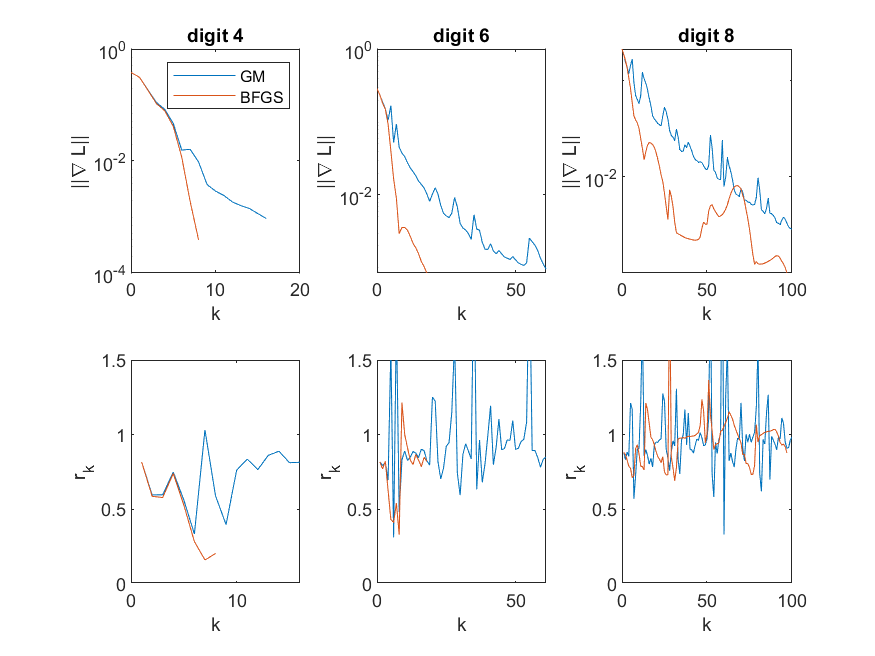
\includegraphics[width=0.9\linewidth]{fig_rk_lambda0.png}
  \caption{Gradient norm (top) and ratio $r_k$ (bottom) for GM (blue) and BFGS (orange) on digits 4, 6 and 8, $\lambda=0$. Values of $r_k$ above 1.5 are cut off.}
  \label{fig:rk}
\end{figure}

For GM, $r_k$ is mostly between 0.8 and 1 in the later iterations and exceeds 1 at times on digits 6 and 8, so the decrease is slow and not monotone. The average reduction per iteration, $(\|\nabla\tilde L(w^{K+1})\|/\|\nabla\tilde L(w^1)\|)^{1/K}$, is 0.69, 0.91 and 0.96 on digits 4, 6 and 8. This is consistent with linear convergence at a rate close to 1. For BFGS the average reduction is 0.42, 0.72 and 0.95. On digit 4, $r_k$ falls to about 0.15 to 0.2 in the last iterations, which is what superlinear convergence looks like, but with only 8 iterations this cannot be stated confidently. On digits 6 and 8, $r_k$ does not tend to 0: it stays around 0.8 (digit 6) and 0.9 (digit 8) up to the last iteration. BFGS therefore does not reach a superlinear regime before the tolerance stops it. We cannot say whether it would with a smaller tolerance.

\subsection{Accuracy}\label{sec:acc}
Table~\ref{tab:acc} shows the final training loss and the training and test accuracies.

\begin{table}[h]
\centering
\small
\setlength{\tabcolsep}{4pt}
\begin{tabular}{c ccc ccc ccc}
\toprule
 & \multicolumn{3}{c}{$\tilde L^*$} & \multicolumn{3}{c}{train acc.\ [\%]} & \multicolumn{3}{c}{test acc.\ [\%]} \\
\cmidrule(lr){2-4}\cmidrule(lr){5-7}\cmidrule(lr){8-10}
Digit & GM & BFGS & SGM & GM & BFGS & SGM & GM & BFGS & SGM \\
\midrule
1 & $6.0\!\cdot\!10^{-4}$ & $6.3\!\cdot\!10^{-4}$ & $5.0\!\cdot\!10^{-4}$ & 100.0 & 100.0 & 100.0 & 99.8 & 99.8 & 100.0 \\
2 & $5.0\!\cdot\!10^{-3}$ & $5.7\!\cdot\!10^{-3}$ & $4.9\!\cdot\!10^{-3}$ & 99.4 & 99.3 & 99.4 & 99.0 & 98.8 & 99.0 \\
3 & $1.6\!\cdot\!10^{-2}$ & $1.4\!\cdot\!10^{-2}$ & $1.6\!\cdot\!10^{-2}$ & 98.1 & 98.3 & 98.0 & 99.4 & 98.6 & 99.4 \\
4 & $1.0\!\cdot\!10^{-3}$ & $1.8\!\cdot\!10^{-4}$ & $1.4\!\cdot\!10^{-4}$ & 100.0 & 100.0 & 100.0 & 100.0 & 100.0 & 100.0 \\
5 & $1.8\!\cdot\!10^{-3}$ & $8.7\!\cdot\!10^{-4}$ & $1.0\!\cdot\!10^{-3}$ & 99.9 & 99.9 & 99.9 & 100.0 & 100.0 & 100.0 \\
6 & $3.6\!\cdot\!10^{-3}$ & $2.8\!\cdot\!10^{-3}$ & $2.8\!\cdot\!10^{-3}$ & 99.7 & 99.6 & 99.7 & 99.0 & 98.6 & 99.2 \\
7 & $1.7\!\cdot\!10^{-3}$ & $1.4\!\cdot\!10^{-3}$ & $1.0\!\cdot\!10^{-3}$ & 99.9 & 99.9 & 99.9 & 99.6 & 99.6 & 99.8 \\
8 & $2.6\!\cdot\!10^{-2}$ & $2.1\!\cdot\!10^{-2}$ & $2.5\!\cdot\!10^{-2}$ & 97.3 & 97.4 & 96.7 & 96.6 & 96.4 & 97.4 \\
9 & $1.3\!\cdot\!10^{-2}$ & $1.2\!\cdot\!10^{-2}$ & $1.5\!\cdot\!10^{-2}$ & 98.5 & 98.4 & 97.9 & 98.4 & 98.2 & 98.6 \\
0 & $6.4\!\cdot\!10^{-3}$ & $5.8\!\cdot\!10^{-3}$ & $5.8\!\cdot\!10^{-3}$ & 99.4 & 99.2 & 99.3 & 99.6 & 99.6 & 99.6 \\
\midrule
Mean & $7.4\!\cdot\!10^{-3}$ & $6.5\!\cdot\!10^{-3}$ & $7.2\!\cdot\!10^{-3}$ & 99.22 & 99.20 & 99.08 & 99.14 & 98.96 & 99.30 \\
\bottomrule
\end{tabular}
\caption{Final training loss and accuracies for $\lambda=0$. The training set is balanced (50\% positives) and the test set has about 10\% positives, so the two accuracy columns are not directly comparable.}
\label{tab:acc}
\end{table}

\textbf{Across algorithms.} All three algorithms reach about 99\% accuracy on both sets (mean test accuracy 99.14\% for GM, 98.96\% for BFGS and 99.30\% for SGM). The differences are very small: 0.34 percentage points between the best and the worst mean, or fewer than two test images per digit. Each digit was run with one seed only, so the differences cannot be separated from sampling noise with this data. We therefore do not rank the algorithms by accuracy.

Two details are worth noting. First, on digits 3, 8 and 9, BFGS has a lower training loss than GM, but not a higher test accuracy ($\tilde L^*$ is $1.4\cdot10^{-2}$ against $1.6\cdot10^{-2}$ on digit 3, with test accuracies of 98.6\% and 99.4\%). The gaps are 1 to 4 test images, so this is not evidence for an effect. Second, SGM has the lowest mean training accuracy (99.08\%) and the highest mean test accuracy. A possible reason is that early stopping acts as a mild regularizer, but SGM also selects its weights on the test loss, which makes its test accuracy slightly optimistic. A fair comparison needs a separate validation set, and we did not use one.

\textbf{Positives and negatives.} Because the test set contains mostly non-target images, we also report the true positive rate (TPR, share of target images recognised) and the true negative rate (TNR) in Table~\ref{tab:tprtnr}. All algorithms recognise at least 95.2\% of the target images and at least 96.5\% of the other images, so the accuracy of about 99\% is not only the effect of the baseline.

\begin{table}[h]
\centering
\small
\setlength{\tabcolsep}{4pt}
\begin{tabular}{c cc ccc ccc}
\toprule
 & & & \multicolumn{3}{c}{TPR [\%]} & \multicolumn{3}{c}{TNR [\%]} \\
\cmidrule(lr){4-6}\cmidrule(lr){7-9}
Digit & \#pos & baseline [\%] & GM & BFGS & SGM & GM & BFGS & SGM \\
\midrule
1 & 66 & 86.8 & 100.0 & 100.0 & 100.0 & 99.8 & 99.8 & 100.0 \\
2 & 51 & 89.8 & 98.0 & 100.0 & 96.1 & 99.1 & 98.7 & 99.3 \\
3 & 52 & 89.6 & 98.1 & 98.1 & 98.1 & 99.6 & 98.7 & 99.6 \\
4 & 59 & 88.2 & 100.0 & 100.0 & 100.0 & 100.0 & 100.0 & 100.0 \\
5 & 41 & 91.8 & 100.0 & 100.0 & 100.0 & 100.0 & 100.0 & 100.0 \\
6 & 46 & 90.8 & 100.0 & 100.0 & 100.0 & 98.9 & 98.5 & 99.1 \\
7 & 46 & 90.8 & 100.0 & 97.8 & 100.0 & 99.6 & 99.8 & 99.8 \\
8 & 42 & 91.6 & 95.2 & 95.2 & 95.2 & 96.7 & 96.5 & 97.6 \\
9 & 48 & 90.4 & 100.0 & 97.9 & 95.8 & 98.2 & 98.2 & 98.9 \\
0 & 49 & 90.2 & 98.0 & 98.0 & 98.0 & 99.8 & 99.8 & 99.8 \\
\bottomrule
\end{tabular}
\caption{Test set ($q=500$) for $\lambda=0$: number of target images, accuracy of the always-negative classifier, and true positive and true negative rates.}
\label{tab:tprtnr}
\end{table}

\textbf{Across digits.} Digit 8 is clearly the hardest: training accuracy 96.7--97.4\% and test accuracy 96.4--97.4\%, with the highest final loss for all three algorithms ($2.1$--$2.6\cdot10^{-2}$). Digits 9 and 3 follow (training accuracy about 98\%), then 0, 2 and 6, and digits 1, 4 and 5 are recognised almost perfectly (test accuracy 99.8--100\%). The digits with the highest final loss (3, 8, 9) are also the ones where GM needed the most iterations. On digit 8 most errors are false positives: only 2 of the 42 target images are missed, but 11 to 16 of the 458 other images are accepted as an 8. Other digits are therefore mistaken for an 8 more often than the reverse. Since the test images are the same for every target, the true digit of each test image is known from the labels of the ten test sets. For GM, 11 of the 15 false positives are 0s, 3s, 6s and 9s (3, 2, 2 and 4). The clean $7\times5$ patterns explain this. Every lit pixel of a 3 is also lit in an 8, a 9 shares 15 of its 16 lit pixels with an 8, and a 0 and a 6 share 14 and 13 of their 16. After blurring, these digits are therefore hard to tell apart from an 8. The same overlap explains why 3 and 9 are the next hardest digits.

Because the test set is about 90\% negatives, test accuracy can exceed training accuracy even when the classifier is not better (digit 3: 98.1\% training, 99.4\% test for GM).

\subsection{Summary for $\lambda=0$}
BFGS converged within 100 iterations on all digits and needed about half the iterations of GM, at the same cost per iteration. GM also converged on all digits, but needed up to 193 iterations. SGM was the fastest in time, by a factor of about 5 against BFGS, but its stopping rule is statistical, it uses the test set, and its solutions are not stationary by the criterion used for the other two methods. All three methods reach about 99\% accuracy with differences inside the noise of the test set, so for $\lambda=0$ the choice between them is decided by computing time and by what is guaranteed about the solution, not by accuracy.

% Sections 3 and 4: regularization and conclusion.
% Include in main.tex with % Sections 3 and 4: regularization and conclusion.
% Include in main.tex with % Sections 3 and 4: regularization and conclusion.
% Include in main.tex with \input{sec_lambda} before \end{document}.
% Needs fig_rk_lambda.png (made by Code/uonn/uo_nn_lambda_analysis.m).

\section{Effect of regularization}\label{sec:lambdapos}

We now compare the runs with $\lambda\in\{0,\,0.01,\,0.5\}$. As in Section~\ref{sec:lambda0}, the iterations, losses, times and accuracies come from the batch, and the other quantities from \texttt{uo\_nn\_\allowbreak lambda\_\allowbreak analysis.m} (Section~1, Experimental setup). Since the number of GM and BFGS iterations depends on the state of the random generator used by the line search, we also give the mean over the batch run and the five repetitions with other states when we compare iteration counts.

\subsection{Global convergence}\label{sec:lambdaglobal}

\textbf{Theory.} For $\lambda>0$ the objective has a property that it lacks for $\lambda=0$: since the data term is non-negative, $\tilde L(w)\ge\frac{\lambda}{2}\|w\|^2$, so $\tilde L(w)\to\infty$ when $\|w\|\to\infty$. GM and BFGS with a Wolfe line search decrease $\tilde L$ at every iteration, so all iterates stay in the level set $\{w:\tilde L(w)\le\tilde L(w^1)=0.25\}$, which gives
\[
  \|w^k\|\le\sqrt{0.5/\lambda}\;=\;7.1 \text{ for } \lambda=0.01,\qquad 1.0 \text{ for } \lambda=0.5 .
\]
The iterates are therefore bounded and the minimum of $\tilde L$ is attained. For $\lambda=0$ there is no such bound. The loss can keep decreasing while $\|w\|$ grows, because the sigmoid only approaches 0 and 1 for arguments of growing size. In addition, $\lambda I$ is added to the Hessian, $\nabla^2\tilde L=\nabla^2 L+\lambda I$, which raises its smallest eigenvalue by $\lambda$ and lowers its condition number. Both effects should make convergence easier as $\lambda$ grows.

\textbf{Observations.} Table~\ref{tab:convlambda} summarizes the convergence for the three values of $\lambda$.

\begin{table}[h]
\centering
\small
\setlength{\tabcolsep}{3pt}
\begin{tabular}{l ccc ccc ccc}
\toprule
 & \multicolumn{3}{c}{GM} & \multicolumn{3}{c}{BFGS} & \multicolumn{3}{c}{SGM} \\
\cmidrule(lr){2-4}\cmidrule(lr){5-7}\cmidrule(lr){8-10}
$\lambda$ & 0 & 0.01 & 0.5 & 0 & 0.01 & 0.5 & 0 & 0.01 & 0.5 \\
\midrule
Mean iter.\ / epochs & 57.3 & 29.5 & 9.4 & 31.6 & 24.2 & 8.0 & 18.3 & 11.2 & 11.3 \\
Max iter.\ / epochs & 100 & 70 & 13 & 97 & 31 & 9 & 100 & 16 & 14 \\
Not converged & 2 & 0 & 0 & 0 & 0 & 0 & 1 & 0 & 0 \\
Mean, 6 gen.\ states & 57.6 & 31.5 & 9.2 & 33.2 & 25.6 & 6.8 & -- & -- & -- \\
Mean $t$ [s] & 3.18 & 1.62 & 0.50 & 1.78 & 1.37 & 0.47 & 0.33 & 0.24 & 0.26 \\
$\|w^*\|$ & 3.6--6.4 & 1.8--2.4 & .29--.44 & 4.6--35 & 1.8--2.5 & .29--.44 & 4.7--9.6 & 1.8--2.7 & .33--.58 \\
Max $\|\nabla\tilde L(w^*)\|$ & $2.8{\cdot}10^{-3}$ & $9.9{\cdot}10^{-4}$ & $7.7{\cdot}10^{-4}$ & $9.9{\cdot}10^{-4}$ & $9.9{\cdot}10^{-4}$ & $7.4{\cdot}10^{-4}$ & $2.5{\cdot}10^{-2}$ & 0.22 & 0.62 \\
\bottomrule
\end{tabular}
\caption{Convergence for the three values of $\lambda$, over the ten digits. Iterations for GM and BFGS, epochs for SGM. ``Not converged'' means the iteration limit was reached with $\|\nabla\tilde L\|>10^{-3}$ (GM, BFGS) or the 100-epoch limit was reached (SGM). The ``6 generator states'' row is the mean over the batch run and the five repetitions with \texttt{rng(1)}--\texttt{rng(5)}.}
\label{tab:convlambda}
\end{table}

\begin{itemize}
  \item \textbf{GM} converges on all digits for both $\lambda>0$, while at $\lambda=0$ it reached the 100-iteration limit on digits 3 and 8. The mean number of iterations halves from $\lambda=0$ to $\lambda=0.01$ and drops by a further factor of three at $\lambda=0.5$. In the repetitions with other generator states, GM at $\lambda=0$ reached the limit in 18 of 60 runs (always on digits 3, 8 and 9), and for $\lambda>0$ it never needed more than 78 iterations.
  \item \textbf{BFGS} converged on all digits for every $\lambda$, but the worst case improves strongly: from 97 iterations at $\lambda=0$ to 31 and 9. The quantities in the global convergence conditions behave in the same way. Over all BFGS iterations, $\kappa(H_k)$ reached up to $1.6\cdot10^{6}$ for $\lambda=0$, but only $1.2\cdot10^{2}$ for $\lambda=0.01$ and $3.3$ for $\lambda=0.5$. The smallest $\cos\theta_k$ was $0.005$, $0.25$ and $0.94$. For $\lambda>0$ the direction is therefore well away from orthogonal to the gradient, and the condition of Section~\ref{sec:global} holds with a large margin. The line search found a strong Wolfe step in every BFGS iteration for $\lambda>0$. For GM it did so in every iteration except 6 of the 162 iterations on digits 3, 8 and 9 with $\lambda=0.01$.
  \item \textbf{The solution becomes well defined.} At $\lambda=0$, GM and BFGS stop at different points: $\|w^*\|$ is 6.0 for GM and 35 for BFGS on digit 2, and the two final losses differ on every digit (Table~\ref{tab:acc}). The Hessian at the BFGS solutions has small negative eigenvalues on six digits (down to $-5.6\cdot10^{-4}$), so these points are not strict minimizers. For $\lambda>0$, GM and BFGS give the same $\tilde L^*$ to three digits and $\|w^*\|$ within 0.03 on every digit, and the smallest Hessian eigenvalue is 0.011--0.013 for $\lambda=0.01$ and 0.51 for $\lambda=0.5$, that is, about $\lambda$. The observed $\|w^*\|$ is also well inside the bound $\sqrt{0.5/\lambda}$ above.
  \item \textbf{SGM} stopped early on all 20 runs with $\lambda>0$, after 6 to 16 epochs, so in the sense of Section~\ref{sec:global} it converged on every digit. The returned points are, however, further from stationary as $\lambda$ grows: $\|\nabla\tilde L(w^*)\|$ on the full training set is at most $2.5\cdot10^{-2}$ for $\lambda=0$, between $2.3\cdot10^{-2}$ and $0.22$ for $\lambda=0.01$, and between 0.35 and 0.62 for $\lambda=0.5$. The reason for $\lambda=0.5$ is discussed in Section~\ref{sec:lambdaacc}.
\end{itemize}

In summary, regularization makes the global convergence of GM and BFGS easier, both in theory (bounded level sets, a positive definite Hessian at the solution) and in the experiments (no iteration limit reached, well-conditioned $H_k$). It does not help SGM in the same way, because its run length is set by early stopping and not by the gradient.

\subsection{Local convergence and speed}\label{sec:lambdalocal}

\textbf{Conditioning.} The condition number of the Hessian at the solution, $\kappa(\nabla^2\tilde L(w^*))$, is $1.7\cdot10^{2}$--$3.0\cdot10^{2}$ at the GM solutions for $\lambda=0$, 17--69 for $\lambda=0.01$ and 3.1--4.1 for $\lambda=0.5$. For GM the theory predicts a linear rate that gets worse as $\kappa$ grows. With an exact line search the bound on the reduction of $\tilde L-\tilde L^*$ per iteration is $\left(\frac{\kappa-1}{\kappa+1}\right)^2$, which is 0.98, 0.92 and 0.36 for $\kappa=250$, 50 and 4. Figure~\ref{fig:rklambda} shows the gradient norm for digits 4, 6 and 8.

\begin{figure}[h]
  \centering
  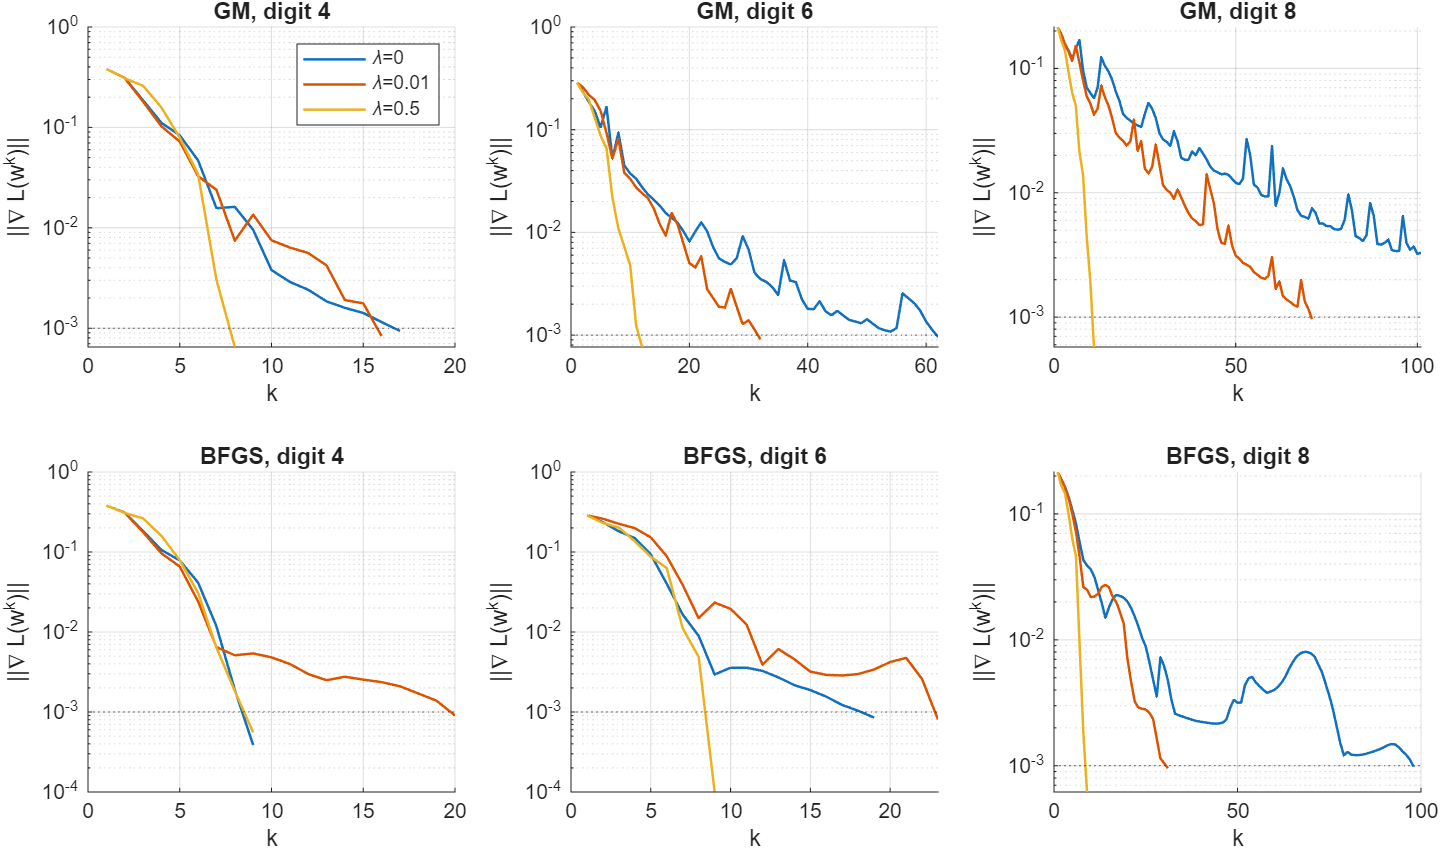
\includegraphics[width=\linewidth]{fig_rk_lambda.png}
  \caption{Gradient norm $\|\nabla\tilde L(w^k)\|$ of GM (top) and BFGS (bottom) on digits 4, 6 and 8, for $\lambda=0$ (blue), $0.01$ (red) and $0.5$ (yellow). The dotted line is the tolerance $10^{-3}$.}
  \label{fig:rklambda}
\end{figure}

\textbf{GM.} The average reduction of the gradient norm per iteration, $(\|\nabla\tilde L(w^{K+1})\|/\|\nabla\tilde L(w^1)\|)^{1/K}$, is on average 0.83 for $\lambda=0$, 0.76 for $\lambda=0.01$ and 0.50 for $\lambda=0.5$ over the ten digits. The ordering is the one predicted by the condition numbers. The observed values are smaller than the bound because the bound is a worst case, and our iterates spend part of the run far from $w^*$. The effect is clearest on digit 8 (Figure~\ref{fig:rklambda}, top right). At $\lambda=0$ the gradient norm still oscillates between $3\cdot10^{-3}$ and $10^{-2}$ after 100 iterations, at $\lambda=0.01$ it decreases more steadily and reaches the tolerance after 70 iterations, and at $\lambda=0.5$ it reaches the tolerance after 10 iterations.

\textbf{BFGS.} For $\lambda=0.5$, BFGS converges in 4 to 12 iterations in all 60 runs, with an average reduction of 0.44 per iteration and a last ratio $r_k$ between 0.02 and 0.34. For $\lambda=0.01$ the average reduction is 0.78, and the median $r_k$ over the last five iterations is 0.87. As for $\lambda=0$ (Section~\ref{sec:local}), we do not see a superlinear phase before the tolerance stops the run.

\textbf{GM against BFGS.} At $\lambda=0$, BFGS needed fewer iterations than GM on all ten digits (mean over the six generator states). At $\lambda=0.5$ this is still the case (6.8 against 9.2 iterations on average). At $\lambda=0.01$, however, BFGS needed fewer iterations only on digits 3, 8, 9 and 0, the four digits with the largest $\kappa(\nabla^2\tilde L(w^*))$ (47 to 69). On the other six digits GM was faster. The largest difference is on digit 7, with 16.2 iterations for GM and 24.7 for BFGS, where $\kappa=21$. On digit 8 the opposite holds, with 69.8 iterations for GM and 29.3 for BFGS. Our explanation is that BFGS mainly helps when the problem is badly conditioned. When $\kappa$ is small, GM is already fast. BFGS starts with $H_1=I$, the same step as GM, and needs several iterations to build a useful approximation of the inverse Hessian. During these iterations its direction deviates from $-\nabla\tilde L$ ($\cos\theta_k$ down to 0.25--0.45 for $\lambda=0.01$) without yet pointing more directly at the minimum. We did not test this explanation, for example with a scaled initial matrix $H_1$.

\textbf{Time.} The time per iteration does not depend on $\lambda$: 0.053 to 0.059\,s per iteration for both GM and BFGS and all three values (total time divided by total iterations). This is expected, since the regularization term only adds $O(n)$ operations to the loss and the gradient. The total time therefore follows the number of iterations, and for GM falls from 3.18\,s to 1.62\,s and 0.50\,s. SGM needs 11 epochs on average for both $\lambda>0$ and takes 0.24 to 0.26\,s, so $\lambda$ has no systematic effect on its run time.

\subsection{Accuracy}\label{sec:lambdaacc}

Table~\ref{tab:acclambda} gives the mean accuracies and the number of test errors, split into false negatives (target images that were rejected) and false positives (other images that were accepted).

\begin{table}[h]
\centering
\small
\setlength{\tabcolsep}{4pt}
\begin{tabular}{l ccc ccc ccc}
\toprule
 & \multicolumn{3}{c}{GM} & \multicolumn{3}{c}{BFGS} & \multicolumn{3}{c}{SGM} \\
\cmidrule(lr){2-4}\cmidrule(lr){5-7}\cmidrule(lr){8-10}
$\lambda$ & 0 & 0.01 & 0.5 & 0 & 0.01 & 0.5 & 0 & 0.01 & 0.5 \\
\midrule
Mean $\tilde L^*$ & 0.0074 & 0.0495 & 0.197 & 0.0065 & 0.0495 & 0.197 & 0.0072 & 0.0589 & 0.295 \\
Mean train acc.\ [\%] & 99.22 & 99.15 & 92.96 & 99.20 & 99.15 & 92.97 & 99.08 & 97.84 & 56.71 \\
Mean test acc.\ [\%] & 99.14 & 99.10 & 87.56 & 98.96 & 99.10 & 87.58 & 99.30 & 99.24 & 91.68 \\
Min test acc.\ [\%] & 96.6 & 96.2 & 64.4 & 96.4 & 96.2 & 64.2 & 97.4 & 98.0 & 89.6 \\
False negatives (of 500) & 5 & 6 & 0 & 6 & 6 & 0 & 8 & 27 & 416 \\
False positives (of 4500) & 38 & 39 & 622 & 46 & 39 & 621 & 27 & 11 & 0 \\
\bottomrule
\end{tabular}
\caption{Accuracy for the three values of $\lambda$, over the ten digits. The test errors are summed over the ten test sets of 500 images, which together contain 500 target and 4500 non-target images. The mean test accuracy of the always-negative classifier is 90.0\%.}
\label{tab:acclambda}
\end{table}

\textbf{$\lambda=0.01$.} The accuracy is practically the same as for $\lambda=0$: the mean test accuracy is 99.10\% for both GM and BFGS, against 99.14\% and 98.96\% without regularization, and the mean training accuracy decreases by less than 0.1 points. On single digits the test accuracy changes by at most 5 images (1 percentage point), and the changes go in both directions. Regularization is meant to reduce overfitting, and at $\lambda=0$ there was little to reduce: the network has only 35 weights for 5000 training samples, and the training and test accuracies were already similar (Section~\ref{sec:acc}). The main effect of $\lambda=0.01$ on accuracy is that GM and BFGS now return the same classifier. At $\lambda=0$ their test accuracies differed by up to 4 images on a digit, at $\lambda=0.01$ they are identical on all ten digits, because both methods find the same minimizer.

SGM behaves differently at $\lambda=0.01$. Its mean training accuracy drops to 97.84\% (93.0\% on digit 8 and 95.3\% on digit 3), while its test accuracy stays at 99.24\%. Its errors move towards false negatives (27 false negatives and 11 false positives, against 8 and 27 at $\lambda=0$). Since SGM selects its weights on the test loss and the test set is 90\% non-target, weights that reject doubtful images are favoured. The test accuracy of SGM should therefore again be read as slightly optimistic.

\textbf{$\lambda=0.5$: GM and BFGS.} Strong regularization makes the classifier clearly worse. The mean test accuracy falls to 87.6\%, which is below the 90.0\% of a classifier that always answers ``not the target''. On digit 8 it is only 64.4\%. All 622 test errors are false positives: no target image is missed, but up to 179 of the 458 non-target images are accepted on digit 8 (true negative rate 61\%). Since the test images are the same for every target, the true digit of each test image is known from the labels of the ten test sets. For target 8, 173 of the 178 false positives are 0s, 3s, 6s and 9s (45, 52, 34 and 42). For target 9 they are 0s, 3s and 8s, and for target 3 they are 2s, 8s and 9s. These are the digits whose $7\times5$ pattern overlaps most with the target (Section~\ref{sec:acc}).

We explain this as follows. With $\lambda=0.5$ the penalty dominates and $\|w^*\|\le0.44$. For small $w$, the optimality condition $\nabla L(w^*)+\lambda w^*=0$ gives $w^*\approx-\frac1\lambda\nabla L(0)$, and since $y(x,0)=\frac12$,
\[
  -\nabla L(0)=\frac{1}{4p}\sum_{j=1}^{p}(2y_j^{TR}-1)\,\sigma(x_j^{TR})\approx\frac18\left(\bar\sigma_{\text{target}}-\bar\sigma_{\text{other}}\right),
\]
where $\bar\sigma$ is the mean of $\sigma(x_j^{TR})$ over the target and the non-target images (the training set is balanced). The weights are then roughly the difference between the average target image and the average other image. Indeed, the cosine between $w^*$ and $-\nabla L(0)$ is 0.90 to 0.999 for $\lambda=0.5$, against 0.68 to 0.99 for $\lambda=0$. Such a template gives a positive score to every image that lights most of the target's pixels, which explains the false positives on the overlapping digits. With smaller $\lambda$ the weights can grow, and large negative weights can be put on the few pixels that separate, for example, an 8 from a 0. Because all errors are false positives, the test accuracy (90\% negatives) is lower than the training accuracy (50\% negatives): 87.6\% against 93.0\%. This gap is caused by the different class balance and is not a sign of overfitting.

\textbf{$\lambda=0.5$: SGM.} SGM fails in the opposite way. On 7 of the 10 digits it accepts no image at all (and only 3 on digit 7), so its test accuracy equals the always-negative baseline (for example 89.6\% on digit 3) and its training accuracy is about 50\%. Its final training loss (0.21--0.42) is higher than that of GM and BFGS (0.17--0.22), and on six digits higher than $\tilde L(0)=0.25$, the loss of the starting point. We see the following reason. The SGM update can be written as
\[
  w^{k+1}=(1-\alpha_k\lambda)\,w^k-\alpha_k\nabla L_{\mathcal B}(w^k).
\]
With $\alpha_0=2$ and $\lambda=0.5$, the factor $1-\alpha_k\lambda$ is 0 at the first iteration and at most 0.3 during the epochs in which the returned weights were found (best epoch 2 to 9, so $k\le4500$ and $\alpha_k\ge1.4$). Each step therefore keeps at most 30\% of the previous weights, and $w^k$ is determined mainly by the gradients of the last few minibatches of 10 images. The averaging of the noisy minibatch gradients, which SGM relies on, does not happen. The cosine between the SGM weights and $-\nabla L(0)$ is between $-0.24$ and $0.86$, so the SGM weights do not have the direction of the regularized minimizer. Early stopping on a test set with 90\% non-target images then selects the epoch with the lowest test loss, which in these runs is a classifier that rejects everything. For $\lambda=0.01$ the factor is at least 0.98 and this problem does not occur. A step size scaled with $\lambda$ (for example $\alpha_0\lambda\ll1$) would probably avoid it, but we did not test this.

\textbf{Across digits.} The order of difficulty of the digits does not change with $\lambda$. Digit 8 has the lowest test accuracy for every $\lambda$ for GM and BFGS (96.2\% at $\lambda=0.01$ and 64.4\% at $\lambda=0.5$), followed by 9 and 3 at $\lambda=0.5$ (74.6\% and 81.0\%). Digits 1 and 4 keep a test accuracy of 99.8\% to 100\% even at $\lambda=0.5$. Presumably their patterns differ enough from the other digits that a template of the average image is enough to recognise them.

\section{Conclusion}\label{sec:conclusion}

The three combinations with $\lambda=0.5$ can be excluded on accuracy alone. With $\lambda=0.5$, GM and BFGS are below the always-negative baseline on average (87.6\%), and SGM recognises no target images on seven digits. With $\lambda=0$ and $\lambda=0.01$ all three methods reach about 99\% test accuracy, and the differences between them are a few test images per digit, within the noise of a single test set. The choice is therefore decided by convergence.

We consider \textbf{BFGS with $\lambda=0.01$} the best combination. Its mean test accuracy is 99.10\%, the same as GM and within the noise of the best value in Table~\ref{tab:acclambda}. It converged on all ten digits in at most 31 iterations (at most 38 over all six generator states) and 1.37\,s on average. Compared with $\lambda=0$, the regularization makes the problem better posed. The iterates are bounded, the solution is a strict minimizer that GM and BFGS both find, the line search satisfies the strong Wolfe conditions at every iteration, and $\kappa(H_k)$ stays below $1.2\cdot10^{2}$ instead of reaching $10^{6}$. Compared with GM at the same $\lambda$, BFGS gives the same classifier, needs 15\% less time on average and is much faster on the hardest digit, 8 (30 against 70 iterations). GM needs fewer iterations on the six easier digits, so the advantage of BFGS comes from the hard digits.

SGM with $\lambda=0.01$ (or $\lambda=0$) is the fastest option, about 5.7 times faster than BFGS (0.24\,s on average), with a mean test accuracy of 99.24\%. We do not choose it because its test accuracy is measured on the same set that selects its weights, its training accuracy is lower (97.84\%), and its solutions are not stationary points. It also fails completely at $\lambda=0.5$ with the step sizes used here. For a training set much larger than our $p=5000$, the cost of the full gradient would grow with $p$ while the cost of an SGM step would not, and SGM would become the preferable method.
 before \end{document}.
% Needs fig_rk_lambda.png (made by Code/uonn/uo_nn_lambda_analysis.m).

\section{Effect of regularization}\label{sec:lambdapos}

We now compare the runs with $\lambda\in\{0,\,0.01,\,0.5\}$. As in Section~\ref{sec:lambda0}, the iterations, losses, times and accuracies come from the batch, and the other quantities from \texttt{uo\_nn\_\allowbreak lambda\_\allowbreak analysis.m} (Section~1, Experimental setup). Since the number of GM and BFGS iterations depends on the state of the random generator used by the line search, we also give the mean over the batch run and the five repetitions with other states when we compare iteration counts.

\subsection{Global convergence}\label{sec:lambdaglobal}

\textbf{Theory.} For $\lambda>0$ the objective has a property that it lacks for $\lambda=0$: since the data term is non-negative, $\tilde L(w)\ge\frac{\lambda}{2}\|w\|^2$, so $\tilde L(w)\to\infty$ when $\|w\|\to\infty$. GM and BFGS with a Wolfe line search decrease $\tilde L$ at every iteration, so all iterates stay in the level set $\{w:\tilde L(w)\le\tilde L(w^1)=0.25\}$, which gives
\[
  \|w^k\|\le\sqrt{0.5/\lambda}\;=\;7.1 \text{ for } \lambda=0.01,\qquad 1.0 \text{ for } \lambda=0.5 .
\]
The iterates are therefore bounded and the minimum of $\tilde L$ is attained. For $\lambda=0$ there is no such bound. The loss can keep decreasing while $\|w\|$ grows, because the sigmoid only approaches 0 and 1 for arguments of growing size. In addition, $\lambda I$ is added to the Hessian, $\nabla^2\tilde L=\nabla^2 L+\lambda I$, which raises its smallest eigenvalue by $\lambda$ and lowers its condition number. Both effects should make convergence easier as $\lambda$ grows.

\textbf{Observations.} Table~\ref{tab:convlambda} summarizes the convergence for the three values of $\lambda$.

\begin{table}[h]
\centering
\small
\setlength{\tabcolsep}{3pt}
\begin{tabular}{l ccc ccc ccc}
\toprule
 & \multicolumn{3}{c}{GM} & \multicolumn{3}{c}{BFGS} & \multicolumn{3}{c}{SGM} \\
\cmidrule(lr){2-4}\cmidrule(lr){5-7}\cmidrule(lr){8-10}
$\lambda$ & 0 & 0.01 & 0.5 & 0 & 0.01 & 0.5 & 0 & 0.01 & 0.5 \\
\midrule
Mean iter.\ / epochs & 57.3 & 29.5 & 9.4 & 31.6 & 24.2 & 8.0 & 18.3 & 11.2 & 11.3 \\
Max iter.\ / epochs & 100 & 70 & 13 & 97 & 31 & 9 & 100 & 16 & 14 \\
Not converged & 2 & 0 & 0 & 0 & 0 & 0 & 1 & 0 & 0 \\
Mean, 6 gen.\ states & 57.6 & 31.5 & 9.2 & 33.2 & 25.6 & 6.8 & -- & -- & -- \\
Mean $t$ [s] & 3.18 & 1.62 & 0.50 & 1.78 & 1.37 & 0.47 & 0.33 & 0.24 & 0.26 \\
$\|w^*\|$ & 3.6--6.4 & 1.8--2.4 & .29--.44 & 4.6--35 & 1.8--2.5 & .29--.44 & 4.7--9.6 & 1.8--2.7 & .33--.58 \\
Max $\|\nabla\tilde L(w^*)\|$ & $2.8{\cdot}10^{-3}$ & $9.9{\cdot}10^{-4}$ & $7.7{\cdot}10^{-4}$ & $9.9{\cdot}10^{-4}$ & $9.9{\cdot}10^{-4}$ & $7.4{\cdot}10^{-4}$ & $2.5{\cdot}10^{-2}$ & 0.22 & 0.62 \\
\bottomrule
\end{tabular}
\caption{Convergence for the three values of $\lambda$, over the ten digits. Iterations for GM and BFGS, epochs for SGM. ``Not converged'' means the iteration limit was reached with $\|\nabla\tilde L\|>10^{-3}$ (GM, BFGS) or the 100-epoch limit was reached (SGM). The ``6 generator states'' row is the mean over the batch run and the five repetitions with \texttt{rng(1)}--\texttt{rng(5)}.}
\label{tab:convlambda}
\end{table}

\begin{itemize}
  \item \textbf{GM} converges on all digits for both $\lambda>0$, while at $\lambda=0$ it reached the 100-iteration limit on digits 3 and 8. The mean number of iterations halves from $\lambda=0$ to $\lambda=0.01$ and drops by a further factor of three at $\lambda=0.5$. In the repetitions with other generator states, GM at $\lambda=0$ reached the limit in 18 of 60 runs (always on digits 3, 8 and 9), and for $\lambda>0$ it never needed more than 78 iterations.
  \item \textbf{BFGS} converged on all digits for every $\lambda$, but the worst case improves strongly: from 97 iterations at $\lambda=0$ to 31 and 9. The quantities in the global convergence conditions behave in the same way. Over all BFGS iterations, $\kappa(H_k)$ reached up to $1.6\cdot10^{6}$ for $\lambda=0$, but only $1.2\cdot10^{2}$ for $\lambda=0.01$ and $3.3$ for $\lambda=0.5$. The smallest $\cos\theta_k$ was $0.005$, $0.25$ and $0.94$. For $\lambda>0$ the direction is therefore well away from orthogonal to the gradient, and the condition of Section~\ref{sec:global} holds with a large margin. The line search found a strong Wolfe step in every BFGS iteration for $\lambda>0$. For GM it did so in every iteration except 6 of the 162 iterations on digits 3, 8 and 9 with $\lambda=0.01$.
  \item \textbf{The solution becomes well defined.} At $\lambda=0$, GM and BFGS stop at different points: $\|w^*\|$ is 6.0 for GM and 35 for BFGS on digit 2, and the two final losses differ on every digit (Table~\ref{tab:acc}). The Hessian at the BFGS solutions has small negative eigenvalues on six digits (down to $-5.6\cdot10^{-4}$), so these points are not strict minimizers. For $\lambda>0$, GM and BFGS give the same $\tilde L^*$ to three digits and $\|w^*\|$ within 0.03 on every digit, and the smallest Hessian eigenvalue is 0.011--0.013 for $\lambda=0.01$ and 0.51 for $\lambda=0.5$, that is, about $\lambda$. The observed $\|w^*\|$ is also well inside the bound $\sqrt{0.5/\lambda}$ above.
  \item \textbf{SGM} stopped early on all 20 runs with $\lambda>0$, after 6 to 16 epochs, so in the sense of Section~\ref{sec:global} it converged on every digit. The returned points are, however, further from stationary as $\lambda$ grows: $\|\nabla\tilde L(w^*)\|$ on the full training set is at most $2.5\cdot10^{-2}$ for $\lambda=0$, between $2.3\cdot10^{-2}$ and $0.22$ for $\lambda=0.01$, and between 0.35 and 0.62 for $\lambda=0.5$. The reason for $\lambda=0.5$ is discussed in Section~\ref{sec:lambdaacc}.
\end{itemize}

In summary, regularization makes the global convergence of GM and BFGS easier, both in theory (bounded level sets, a positive definite Hessian at the solution) and in the experiments (no iteration limit reached, well-conditioned $H_k$). It does not help SGM in the same way, because its run length is set by early stopping and not by the gradient.

\subsection{Local convergence and speed}\label{sec:lambdalocal}

\textbf{Conditioning.} The condition number of the Hessian at the solution, $\kappa(\nabla^2\tilde L(w^*))$, is $1.7\cdot10^{2}$--$3.0\cdot10^{2}$ at the GM solutions for $\lambda=0$, 17--69 for $\lambda=0.01$ and 3.1--4.1 for $\lambda=0.5$. For GM the theory predicts a linear rate that gets worse as $\kappa$ grows. With an exact line search the bound on the reduction of $\tilde L-\tilde L^*$ per iteration is $\left(\frac{\kappa-1}{\kappa+1}\right)^2$, which is 0.98, 0.92 and 0.36 for $\kappa=250$, 50 and 4. Figure~\ref{fig:rklambda} shows the gradient norm for digits 4, 6 and 8.

\begin{figure}[h]
  \centering
  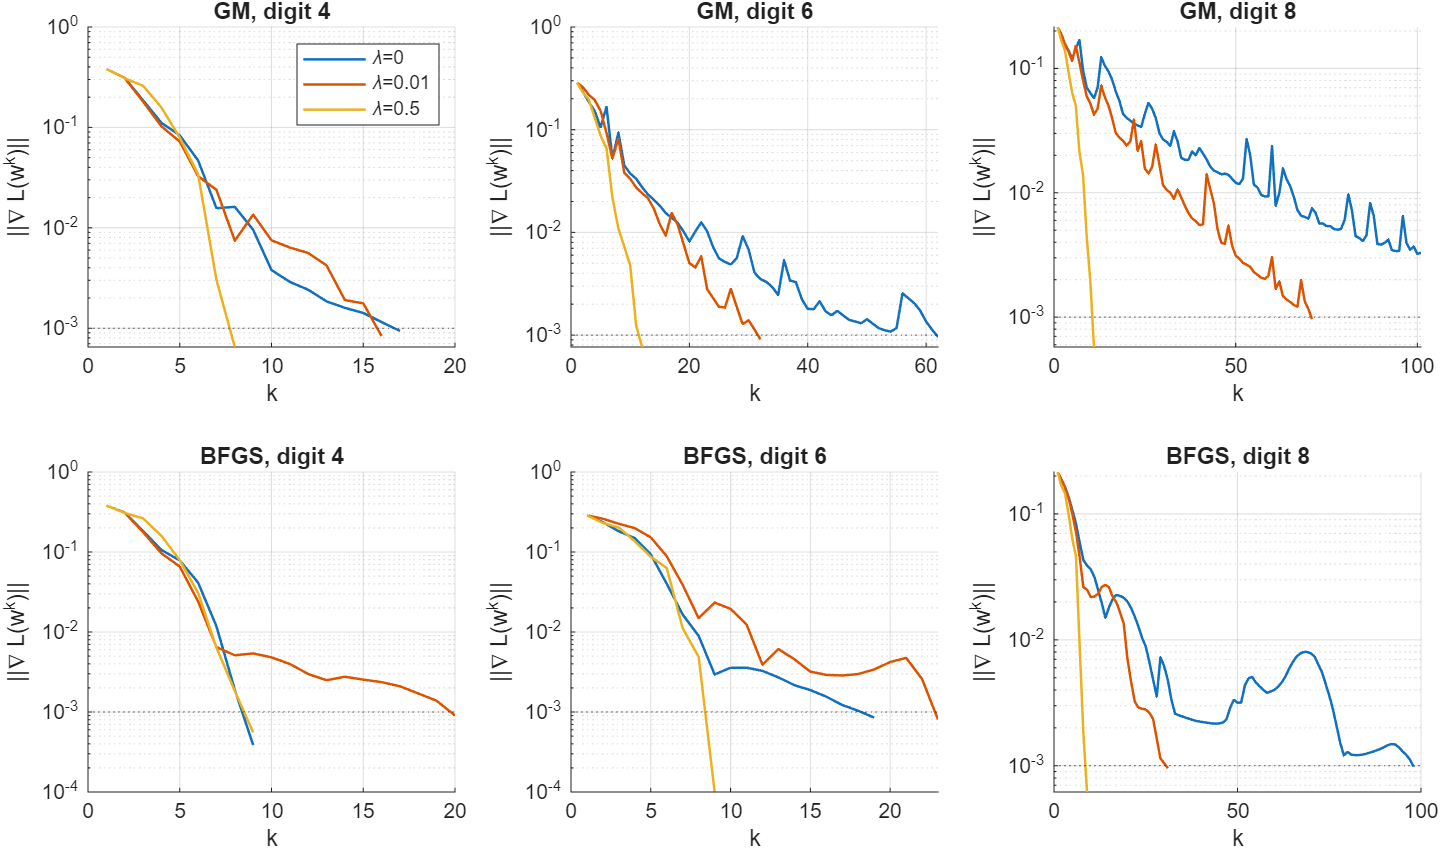
\includegraphics[width=\linewidth]{fig_rk_lambda.png}
  \caption{Gradient norm $\|\nabla\tilde L(w^k)\|$ of GM (top) and BFGS (bottom) on digits 4, 6 and 8, for $\lambda=0$ (blue), $0.01$ (red) and $0.5$ (yellow). The dotted line is the tolerance $10^{-3}$.}
  \label{fig:rklambda}
\end{figure}

\textbf{GM.} The average reduction of the gradient norm per iteration, $(\|\nabla\tilde L(w^{K+1})\|/\|\nabla\tilde L(w^1)\|)^{1/K}$, is on average 0.83 for $\lambda=0$, 0.76 for $\lambda=0.01$ and 0.50 for $\lambda=0.5$ over the ten digits. The ordering is the one predicted by the condition numbers. The observed values are smaller than the bound because the bound is a worst case, and our iterates spend part of the run far from $w^*$. The effect is clearest on digit 8 (Figure~\ref{fig:rklambda}, top right). At $\lambda=0$ the gradient norm still oscillates between $3\cdot10^{-3}$ and $10^{-2}$ after 100 iterations, at $\lambda=0.01$ it decreases more steadily and reaches the tolerance after 70 iterations, and at $\lambda=0.5$ it reaches the tolerance after 10 iterations.

\textbf{BFGS.} For $\lambda=0.5$, BFGS converges in 4 to 12 iterations in all 60 runs, with an average reduction of 0.44 per iteration and a last ratio $r_k$ between 0.02 and 0.34. For $\lambda=0.01$ the average reduction is 0.78, and the median $r_k$ over the last five iterations is 0.87. As for $\lambda=0$ (Section~\ref{sec:local}), we do not see a superlinear phase before the tolerance stops the run.

\textbf{GM against BFGS.} At $\lambda=0$, BFGS needed fewer iterations than GM on all ten digits (mean over the six generator states). At $\lambda=0.5$ this is still the case (6.8 against 9.2 iterations on average). At $\lambda=0.01$, however, BFGS needed fewer iterations only on digits 3, 8, 9 and 0, the four digits with the largest $\kappa(\nabla^2\tilde L(w^*))$ (47 to 69). On the other six digits GM was faster. The largest difference is on digit 7, with 16.2 iterations for GM and 24.7 for BFGS, where $\kappa=21$. On digit 8 the opposite holds, with 69.8 iterations for GM and 29.3 for BFGS. Our explanation is that BFGS mainly helps when the problem is badly conditioned. When $\kappa$ is small, GM is already fast. BFGS starts with $H_1=I$, the same step as GM, and needs several iterations to build a useful approximation of the inverse Hessian. During these iterations its direction deviates from $-\nabla\tilde L$ ($\cos\theta_k$ down to 0.25--0.45 for $\lambda=0.01$) without yet pointing more directly at the minimum. We did not test this explanation, for example with a scaled initial matrix $H_1$.

\textbf{Time.} The time per iteration does not depend on $\lambda$: 0.053 to 0.059\,s per iteration for both GM and BFGS and all three values (total time divided by total iterations). This is expected, since the regularization term only adds $O(n)$ operations to the loss and the gradient. The total time therefore follows the number of iterations, and for GM falls from 3.18\,s to 1.62\,s and 0.50\,s. SGM needs 11 epochs on average for both $\lambda>0$ and takes 0.24 to 0.26\,s, so $\lambda$ has no systematic effect on its run time.

\subsection{Accuracy}\label{sec:lambdaacc}

Table~\ref{tab:acclambda} gives the mean accuracies and the number of test errors, split into false negatives (target images that were rejected) and false positives (other images that were accepted).

\begin{table}[h]
\centering
\small
\setlength{\tabcolsep}{4pt}
\begin{tabular}{l ccc ccc ccc}
\toprule
 & \multicolumn{3}{c}{GM} & \multicolumn{3}{c}{BFGS} & \multicolumn{3}{c}{SGM} \\
\cmidrule(lr){2-4}\cmidrule(lr){5-7}\cmidrule(lr){8-10}
$\lambda$ & 0 & 0.01 & 0.5 & 0 & 0.01 & 0.5 & 0 & 0.01 & 0.5 \\
\midrule
Mean $\tilde L^*$ & 0.0074 & 0.0495 & 0.197 & 0.0065 & 0.0495 & 0.197 & 0.0072 & 0.0589 & 0.295 \\
Mean train acc.\ [\%] & 99.22 & 99.15 & 92.96 & 99.20 & 99.15 & 92.97 & 99.08 & 97.84 & 56.71 \\
Mean test acc.\ [\%] & 99.14 & 99.10 & 87.56 & 98.96 & 99.10 & 87.58 & 99.30 & 99.24 & 91.68 \\
Min test acc.\ [\%] & 96.6 & 96.2 & 64.4 & 96.4 & 96.2 & 64.2 & 97.4 & 98.0 & 89.6 \\
False negatives (of 500) & 5 & 6 & 0 & 6 & 6 & 0 & 8 & 27 & 416 \\
False positives (of 4500) & 38 & 39 & 622 & 46 & 39 & 621 & 27 & 11 & 0 \\
\bottomrule
\end{tabular}
\caption{Accuracy for the three values of $\lambda$, over the ten digits. The test errors are summed over the ten test sets of 500 images, which together contain 500 target and 4500 non-target images. The mean test accuracy of the always-negative classifier is 90.0\%.}
\label{tab:acclambda}
\end{table}

\textbf{$\lambda=0.01$.} The accuracy is practically the same as for $\lambda=0$: the mean test accuracy is 99.10\% for both GM and BFGS, against 99.14\% and 98.96\% without regularization, and the mean training accuracy decreases by less than 0.1 points. On single digits the test accuracy changes by at most 5 images (1 percentage point), and the changes go in both directions. Regularization is meant to reduce overfitting, and at $\lambda=0$ there was little to reduce: the network has only 35 weights for 5000 training samples, and the training and test accuracies were already similar (Section~\ref{sec:acc}). The main effect of $\lambda=0.01$ on accuracy is that GM and BFGS now return the same classifier. At $\lambda=0$ their test accuracies differed by up to 4 images on a digit, at $\lambda=0.01$ they are identical on all ten digits, because both methods find the same minimizer.

SGM behaves differently at $\lambda=0.01$. Its mean training accuracy drops to 97.84\% (93.0\% on digit 8 and 95.3\% on digit 3), while its test accuracy stays at 99.24\%. Its errors move towards false negatives (27 false negatives and 11 false positives, against 8 and 27 at $\lambda=0$). Since SGM selects its weights on the test loss and the test set is 90\% non-target, weights that reject doubtful images are favoured. The test accuracy of SGM should therefore again be read as slightly optimistic.

\textbf{$\lambda=0.5$: GM and BFGS.} Strong regularization makes the classifier clearly worse. The mean test accuracy falls to 87.6\%, which is below the 90.0\% of a classifier that always answers ``not the target''. On digit 8 it is only 64.4\%. All 622 test errors are false positives: no target image is missed, but up to 179 of the 458 non-target images are accepted on digit 8 (true negative rate 61\%). Since the test images are the same for every target, the true digit of each test image is known from the labels of the ten test sets. For target 8, 173 of the 178 false positives are 0s, 3s, 6s and 9s (45, 52, 34 and 42). For target 9 they are 0s, 3s and 8s, and for target 3 they are 2s, 8s and 9s. These are the digits whose $7\times5$ pattern overlaps most with the target (Section~\ref{sec:acc}).

We explain this as follows. With $\lambda=0.5$ the penalty dominates and $\|w^*\|\le0.44$. For small $w$, the optimality condition $\nabla L(w^*)+\lambda w^*=0$ gives $w^*\approx-\frac1\lambda\nabla L(0)$, and since $y(x,0)=\frac12$,
\[
  -\nabla L(0)=\frac{1}{4p}\sum_{j=1}^{p}(2y_j^{TR}-1)\,\sigma(x_j^{TR})\approx\frac18\left(\bar\sigma_{\text{target}}-\bar\sigma_{\text{other}}\right),
\]
where $\bar\sigma$ is the mean of $\sigma(x_j^{TR})$ over the target and the non-target images (the training set is balanced). The weights are then roughly the difference between the average target image and the average other image. Indeed, the cosine between $w^*$ and $-\nabla L(0)$ is 0.90 to 0.999 for $\lambda=0.5$, against 0.68 to 0.99 for $\lambda=0$. Such a template gives a positive score to every image that lights most of the target's pixels, which explains the false positives on the overlapping digits. With smaller $\lambda$ the weights can grow, and large negative weights can be put on the few pixels that separate, for example, an 8 from a 0. Because all errors are false positives, the test accuracy (90\% negatives) is lower than the training accuracy (50\% negatives): 87.6\% against 93.0\%. This gap is caused by the different class balance and is not a sign of overfitting.

\textbf{$\lambda=0.5$: SGM.} SGM fails in the opposite way. On 7 of the 10 digits it accepts no image at all (and only 3 on digit 7), so its test accuracy equals the always-negative baseline (for example 89.6\% on digit 3) and its training accuracy is about 50\%. Its final training loss (0.21--0.42) is higher than that of GM and BFGS (0.17--0.22), and on six digits higher than $\tilde L(0)=0.25$, the loss of the starting point. We see the following reason. The SGM update can be written as
\[
  w^{k+1}=(1-\alpha_k\lambda)\,w^k-\alpha_k\nabla L_{\mathcal B}(w^k).
\]
With $\alpha_0=2$ and $\lambda=0.5$, the factor $1-\alpha_k\lambda$ is 0 at the first iteration and at most 0.3 during the epochs in which the returned weights were found (best epoch 2 to 9, so $k\le4500$ and $\alpha_k\ge1.4$). Each step therefore keeps at most 30\% of the previous weights, and $w^k$ is determined mainly by the gradients of the last few minibatches of 10 images. The averaging of the noisy minibatch gradients, which SGM relies on, does not happen. The cosine between the SGM weights and $-\nabla L(0)$ is between $-0.24$ and $0.86$, so the SGM weights do not have the direction of the regularized minimizer. Early stopping on a test set with 90\% non-target images then selects the epoch with the lowest test loss, which in these runs is a classifier that rejects everything. For $\lambda=0.01$ the factor is at least 0.98 and this problem does not occur. A step size scaled with $\lambda$ (for example $\alpha_0\lambda\ll1$) would probably avoid it, but we did not test this.

\textbf{Across digits.} The order of difficulty of the digits does not change with $\lambda$. Digit 8 has the lowest test accuracy for every $\lambda$ for GM and BFGS (96.2\% at $\lambda=0.01$ and 64.4\% at $\lambda=0.5$), followed by 9 and 3 at $\lambda=0.5$ (74.6\% and 81.0\%). Digits 1 and 4 keep a test accuracy of 99.8\% to 100\% even at $\lambda=0.5$. Presumably their patterns differ enough from the other digits that a template of the average image is enough to recognise them.

\section{Conclusion}\label{sec:conclusion}

The three combinations with $\lambda=0.5$ can be excluded on accuracy alone. With $\lambda=0.5$, GM and BFGS are below the always-negative baseline on average (87.6\%), and SGM recognises no target images on seven digits. With $\lambda=0$ and $\lambda=0.01$ all three methods reach about 99\% test accuracy, and the differences between them are a few test images per digit, within the noise of a single test set. The choice is therefore decided by convergence.

We consider \textbf{BFGS with $\lambda=0.01$} the best combination. Its mean test accuracy is 99.10\%, the same as GM and within the noise of the best value in Table~\ref{tab:acclambda}. It converged on all ten digits in at most 31 iterations (at most 38 over all six generator states) and 1.37\,s on average. Compared with $\lambda=0$, the regularization makes the problem better posed. The iterates are bounded, the solution is a strict minimizer that GM and BFGS both find, the line search satisfies the strong Wolfe conditions at every iteration, and $\kappa(H_k)$ stays below $1.2\cdot10^{2}$ instead of reaching $10^{6}$. Compared with GM at the same $\lambda$, BFGS gives the same classifier, needs 15\% less time on average and is much faster on the hardest digit, 8 (30 against 70 iterations). GM needs fewer iterations on the six easier digits, so the advantage of BFGS comes from the hard digits.

SGM with $\lambda=0.01$ (or $\lambda=0$) is the fastest option, about 5.7 times faster than BFGS (0.24\,s on average), with a mean test accuracy of 99.24\%. We do not choose it because its test accuracy is measured on the same set that selects its weights, its training accuracy is lower (97.84\%), and its solutions are not stationary points. It also fails completely at $\lambda=0.5$ with the step sizes used here. For a training set much larger than our $p=5000$, the cost of the full gradient would grow with $p$ while the cost of an SGM step would not, and SGM would become the preferable method.
 before \end{document}.
% Needs fig_rk_lambda.png (made by Code/uonn/uo_nn_lambda_analysis.m).

\section{Effect of regularization}\label{sec:lambdapos}

We now compare the runs with $\lambda\in\{0,\,0.01,\,0.5\}$. As in Section~\ref{sec:lambda0}, the iterations, losses, times and accuracies come from the batch, and the other quantities from \texttt{uo\_nn\_\allowbreak lambda\_\allowbreak analysis.m} (Section~1, Experimental setup). Since the number of GM and BFGS iterations depends on the state of the random generator used by the line search, we also give the mean over the batch run and the five repetitions with other states when we compare iteration counts.

\subsection{Global convergence}\label{sec:lambdaglobal}

\textbf{Theory.} For $\lambda>0$ the objective has a property that it lacks for $\lambda=0$: since the data term is non-negative, $\tilde L(w)\ge\frac{\lambda}{2}\|w\|^2$, so $\tilde L(w)\to\infty$ when $\|w\|\to\infty$. GM and BFGS with a Wolfe line search decrease $\tilde L$ at every iteration, so all iterates stay in the level set $\{w:\tilde L(w)\le\tilde L(w^1)=0.25\}$, which gives
\[
  \|w^k\|\le\sqrt{0.5/\lambda}\;=\;7.1 \text{ for } \lambda=0.01,\qquad 1.0 \text{ for } \lambda=0.5 .
\]
The iterates are therefore bounded and the minimum of $\tilde L$ is attained. For $\lambda=0$ there is no such bound. The loss can keep decreasing while $\|w\|$ grows, because the sigmoid only approaches 0 and 1 for arguments of growing size. In addition, $\lambda I$ is added to the Hessian, $\nabla^2\tilde L=\nabla^2 L+\lambda I$, which raises its smallest eigenvalue by $\lambda$ and lowers its condition number. Both effects should make convergence easier as $\lambda$ grows.

\textbf{Observations.} Table~\ref{tab:convlambda} summarizes the convergence for the three values of $\lambda$.

\begin{table}[h]
\centering
\small
\setlength{\tabcolsep}{3pt}
\begin{tabular}{l ccc ccc ccc}
\toprule
 & \multicolumn{3}{c}{GM} & \multicolumn{3}{c}{BFGS} & \multicolumn{3}{c}{SGM} \\
\cmidrule(lr){2-4}\cmidrule(lr){5-7}\cmidrule(lr){8-10}
$\lambda$ & 0 & 0.01 & 0.5 & 0 & 0.01 & 0.5 & 0 & 0.01 & 0.5 \\
\midrule
Mean iter.\ / epochs & 57.3 & 29.5 & 9.4 & 31.6 & 24.2 & 8.0 & 18.3 & 11.2 & 11.3 \\
Max iter.\ / epochs & 100 & 70 & 13 & 97 & 31 & 9 & 100 & 16 & 14 \\
Not converged & 2 & 0 & 0 & 0 & 0 & 0 & 1 & 0 & 0 \\
Mean, 6 gen.\ states & 57.6 & 31.5 & 9.2 & 33.2 & 25.6 & 6.8 & -- & -- & -- \\
Mean $t$ [s] & 3.18 & 1.62 & 0.50 & 1.78 & 1.37 & 0.47 & 0.33 & 0.24 & 0.26 \\
$\|w^*\|$ & 3.6--6.4 & 1.8--2.4 & .29--.44 & 4.6--35 & 1.8--2.5 & .29--.44 & 4.7--9.6 & 1.8--2.7 & .33--.58 \\
Max $\|\nabla\tilde L(w^*)\|$ & $2.8{\cdot}10^{-3}$ & $9.9{\cdot}10^{-4}$ & $7.7{\cdot}10^{-4}$ & $9.9{\cdot}10^{-4}$ & $9.9{\cdot}10^{-4}$ & $7.4{\cdot}10^{-4}$ & $2.5{\cdot}10^{-2}$ & 0.22 & 0.62 \\
\bottomrule
\end{tabular}
\caption{Convergence for the three values of $\lambda$, over the ten digits. Iterations for GM and BFGS, epochs for SGM. ``Not converged'' means the iteration limit was reached with $\|\nabla\tilde L\|>10^{-3}$ (GM, BFGS) or the 100-epoch limit was reached (SGM). The ``6 generator states'' row is the mean over the batch run and the five repetitions with \texttt{rng(1)}--\texttt{rng(5)}.}
\label{tab:convlambda}
\end{table}

\begin{itemize}
  \item \textbf{GM} converges on all digits for both $\lambda>0$, while at $\lambda=0$ it reached the 100-iteration limit on digits 3 and 8. The mean number of iterations halves from $\lambda=0$ to $\lambda=0.01$ and drops by a further factor of three at $\lambda=0.5$. In the repetitions with other generator states, GM at $\lambda=0$ reached the limit in 18 of 60 runs (always on digits 3, 8 and 9), and for $\lambda>0$ it never needed more than 78 iterations.
  \item \textbf{BFGS} converged on all digits for every $\lambda$, but the worst case improves strongly: from 97 iterations at $\lambda=0$ to 31 and 9. The quantities in the global convergence conditions behave in the same way. Over all BFGS iterations, $\kappa(H_k)$ reached up to $1.6\cdot10^{6}$ for $\lambda=0$, but only $1.2\cdot10^{2}$ for $\lambda=0.01$ and $3.3$ for $\lambda=0.5$. The smallest $\cos\theta_k$ was $0.005$, $0.25$ and $0.94$. For $\lambda>0$ the direction is therefore well away from orthogonal to the gradient, and the condition of Section~\ref{sec:global} holds with a large margin. The line search found a strong Wolfe step in every BFGS iteration for $\lambda>0$. For GM it did so in every iteration except 6 of the 162 iterations on digits 3, 8 and 9 with $\lambda=0.01$.
  \item \textbf{The solution becomes well defined.} At $\lambda=0$, GM and BFGS stop at different points: $\|w^*\|$ is 6.0 for GM and 35 for BFGS on digit 2, and the two final losses differ on every digit (Table~\ref{tab:acc}). The Hessian at the BFGS solutions has small negative eigenvalues on six digits (down to $-5.6\cdot10^{-4}$), so these points are not strict minimizers. For $\lambda>0$, GM and BFGS give the same $\tilde L^*$ to three digits and $\|w^*\|$ within 0.03 on every digit, and the smallest Hessian eigenvalue is 0.011--0.013 for $\lambda=0.01$ and 0.51 for $\lambda=0.5$, that is, about $\lambda$. The observed $\|w^*\|$ is also well inside the bound $\sqrt{0.5/\lambda}$ above.
  \item \textbf{SGM} stopped early on all 20 runs with $\lambda>0$, after 6 to 16 epochs, so in the sense of Section~\ref{sec:global} it converged on every digit. The returned points are, however, further from stationary as $\lambda$ grows: $\|\nabla\tilde L(w^*)\|$ on the full training set is at most $2.5\cdot10^{-2}$ for $\lambda=0$, between $2.3\cdot10^{-2}$ and $0.22$ for $\lambda=0.01$, and between 0.35 and 0.62 for $\lambda=0.5$. The reason for $\lambda=0.5$ is discussed in Section~\ref{sec:lambdaacc}.
\end{itemize}

In summary, regularization makes the global convergence of GM and BFGS easier, both in theory (bounded level sets, a positive definite Hessian at the solution) and in the experiments (no iteration limit reached, well-conditioned $H_k$). It does not help SGM in the same way, because its run length is set by early stopping and not by the gradient.

\subsection{Local convergence and speed}\label{sec:lambdalocal}

\textbf{Conditioning.} The condition number of the Hessian at the solution, $\kappa(\nabla^2\tilde L(w^*))$, is $1.7\cdot10^{2}$--$3.0\cdot10^{2}$ at the GM solutions for $\lambda=0$, 17--69 for $\lambda=0.01$ and 3.1--4.1 for $\lambda=0.5$. For GM the theory predicts a linear rate that gets worse as $\kappa$ grows. With an exact line search the bound on the reduction of $\tilde L-\tilde L^*$ per iteration is $\left(\frac{\kappa-1}{\kappa+1}\right)^2$, which is 0.98, 0.92 and 0.36 for $\kappa=250$, 50 and 4. Figure~\ref{fig:rklambda} shows the gradient norm for digits 4, 6 and 8.

\begin{figure}[h]
  \centering
  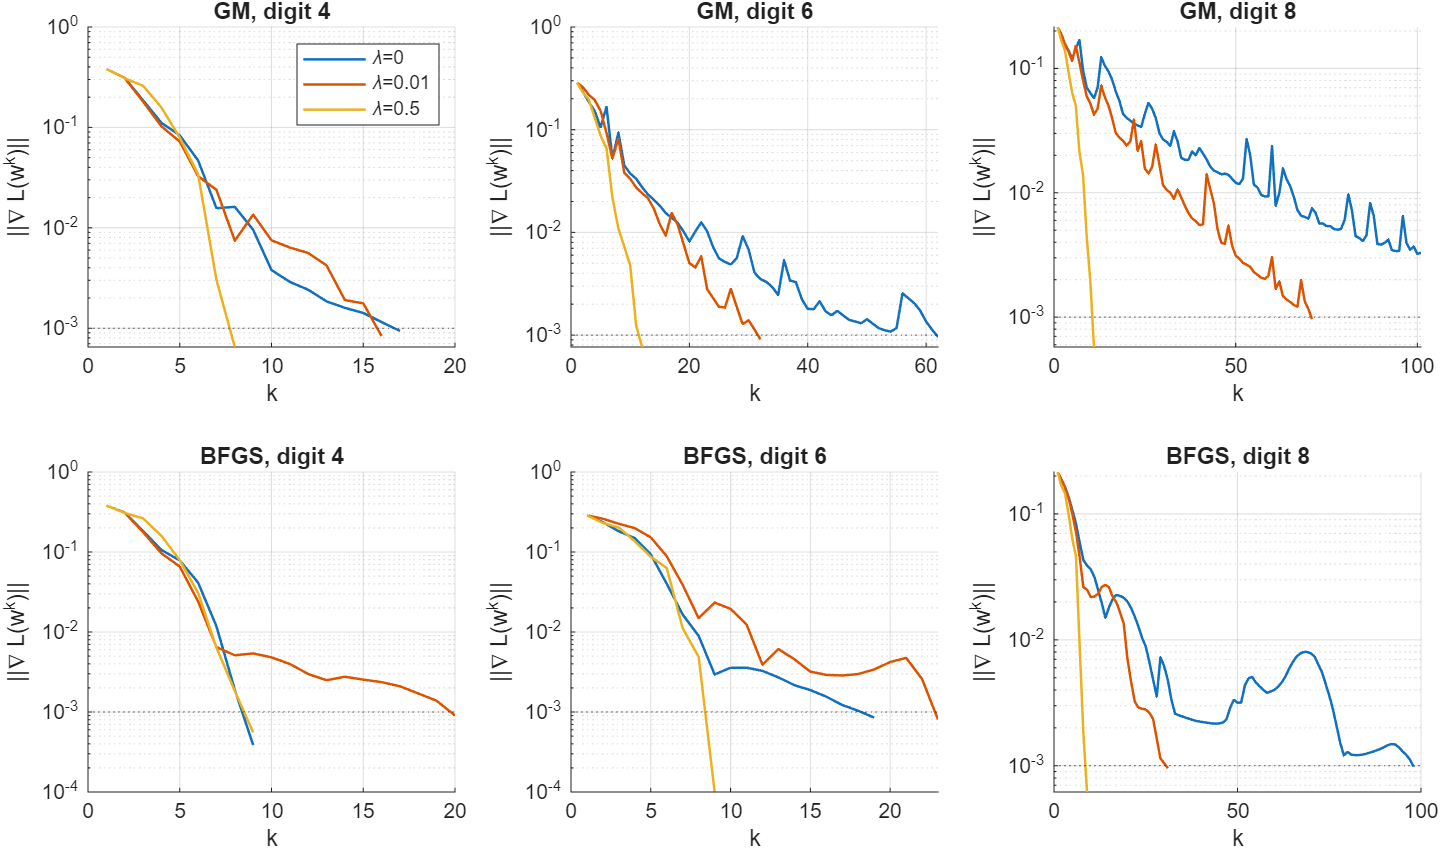
\includegraphics[width=\linewidth]{fig_rk_lambda.png}
  \caption{Gradient norm $\|\nabla\tilde L(w^k)\|$ of GM (top) and BFGS (bottom) on digits 4, 6 and 8, for $\lambda=0$ (blue), $0.01$ (red) and $0.5$ (yellow). The dotted line is the tolerance $10^{-3}$.}
  \label{fig:rklambda}
\end{figure}

\textbf{GM.} The average reduction of the gradient norm per iteration, $(\|\nabla\tilde L(w^{K+1})\|/\|\nabla\tilde L(w^1)\|)^{1/K}$, is on average 0.83 for $\lambda=0$, 0.76 for $\lambda=0.01$ and 0.50 for $\lambda=0.5$ over the ten digits. The ordering is the one predicted by the condition numbers. The observed values are smaller than the bound because the bound is a worst case, and our iterates spend part of the run far from $w^*$. The effect is clearest on digit 8 (Figure~\ref{fig:rklambda}, top right). At $\lambda=0$ the gradient norm still oscillates between $3\cdot10^{-3}$ and $10^{-2}$ after 100 iterations, at $\lambda=0.01$ it decreases more steadily and reaches the tolerance after 70 iterations, and at $\lambda=0.5$ it reaches the tolerance after 10 iterations.

\textbf{BFGS.} For $\lambda=0.5$, BFGS converges in 4 to 12 iterations in all 60 runs, with an average reduction of 0.44 per iteration and a last ratio $r_k$ between 0.02 and 0.34. For $\lambda=0.01$ the average reduction is 0.78, and the median $r_k$ over the last five iterations is 0.87. As for $\lambda=0$ (Section~\ref{sec:local}), we do not see a superlinear phase before the tolerance stops the run.

\textbf{GM against BFGS.} At $\lambda=0$, BFGS needed fewer iterations than GM on all ten digits (mean over the six generator states). At $\lambda=0.5$ this is still the case (6.8 against 9.2 iterations on average). At $\lambda=0.01$, however, BFGS needed fewer iterations only on digits 3, 8, 9 and 0, the four digits with the largest $\kappa(\nabla^2\tilde L(w^*))$ (47 to 69). On the other six digits GM was faster. The largest difference is on digit 7, with 16.2 iterations for GM and 24.7 for BFGS, where $\kappa=21$. On digit 8 the opposite holds, with 69.8 iterations for GM and 29.3 for BFGS. Our explanation is that BFGS mainly helps when the problem is badly conditioned. When $\kappa$ is small, GM is already fast. BFGS starts with $H_1=I$, the same step as GM, and needs several iterations to build a useful approximation of the inverse Hessian. During these iterations its direction deviates from $-\nabla\tilde L$ ($\cos\theta_k$ down to 0.25--0.45 for $\lambda=0.01$) without yet pointing more directly at the minimum. We did not test this explanation, for example with a scaled initial matrix $H_1$.

\textbf{Time.} The time per iteration does not depend on $\lambda$: 0.053 to 0.059\,s per iteration for both GM and BFGS and all three values (total time divided by total iterations). This is expected, since the regularization term only adds $O(n)$ operations to the loss and the gradient. The total time therefore follows the number of iterations, and for GM falls from 3.18\,s to 1.62\,s and 0.50\,s. SGM needs 11 epochs on average for both $\lambda>0$ and takes 0.24 to 0.26\,s, so $\lambda$ has no systematic effect on its run time.

\subsection{Accuracy}\label{sec:lambdaacc}

Table~\ref{tab:acclambda} gives the mean accuracies and the number of test errors, split into false negatives (target images that were rejected) and false positives (other images that were accepted).

\begin{table}[h]
\centering
\small
\setlength{\tabcolsep}{4pt}
\begin{tabular}{l ccc ccc ccc}
\toprule
 & \multicolumn{3}{c}{GM} & \multicolumn{3}{c}{BFGS} & \multicolumn{3}{c}{SGM} \\
\cmidrule(lr){2-4}\cmidrule(lr){5-7}\cmidrule(lr){8-10}
$\lambda$ & 0 & 0.01 & 0.5 & 0 & 0.01 & 0.5 & 0 & 0.01 & 0.5 \\
\midrule
Mean $\tilde L^*$ & 0.0074 & 0.0495 & 0.197 & 0.0065 & 0.0495 & 0.197 & 0.0072 & 0.0589 & 0.295 \\
Mean train acc.\ [\%] & 99.22 & 99.15 & 92.96 & 99.20 & 99.15 & 92.97 & 99.08 & 97.84 & 56.71 \\
Mean test acc.\ [\%] & 99.14 & 99.10 & 87.56 & 98.96 & 99.10 & 87.58 & 99.30 & 99.24 & 91.68 \\
Min test acc.\ [\%] & 96.6 & 96.2 & 64.4 & 96.4 & 96.2 & 64.2 & 97.4 & 98.0 & 89.6 \\
False negatives (of 500) & 5 & 6 & 0 & 6 & 6 & 0 & 8 & 27 & 416 \\
False positives (of 4500) & 38 & 39 & 622 & 46 & 39 & 621 & 27 & 11 & 0 \\
\bottomrule
\end{tabular}
\caption{Accuracy for the three values of $\lambda$, over the ten digits. The test errors are summed over the ten test sets of 500 images, which together contain 500 target and 4500 non-target images. The mean test accuracy of the always-negative classifier is 90.0\%.}
\label{tab:acclambda}
\end{table}

\textbf{$\lambda=0.01$.} The accuracy is practically the same as for $\lambda=0$: the mean test accuracy is 99.10\% for both GM and BFGS, against 99.14\% and 98.96\% without regularization, and the mean training accuracy decreases by less than 0.1 points. On single digits the test accuracy changes by at most 5 images (1 percentage point), and the changes go in both directions. Regularization is meant to reduce overfitting, and at $\lambda=0$ there was little to reduce: the network has only 35 weights for 5000 training samples, and the training and test accuracies were already similar (Section~\ref{sec:acc}). The main effect of $\lambda=0.01$ on accuracy is that GM and BFGS now return the same classifier. At $\lambda=0$ their test accuracies differed by up to 4 images on a digit, at $\lambda=0.01$ they are identical on all ten digits, because both methods find the same minimizer.

SGM behaves differently at $\lambda=0.01$. Its mean training accuracy drops to 97.84\% (93.0\% on digit 8 and 95.3\% on digit 3), while its test accuracy stays at 99.24\%. Its errors move towards false negatives (27 false negatives and 11 false positives, against 8 and 27 at $\lambda=0$). Since SGM selects its weights on the test loss and the test set is 90\% non-target, weights that reject doubtful images are favoured. The test accuracy of SGM should therefore again be read as slightly optimistic.

\textbf{$\lambda=0.5$: GM and BFGS.} Strong regularization makes the classifier clearly worse. The mean test accuracy falls to 87.6\%, which is below the 90.0\% of a classifier that always answers ``not the target''. On digit 8 it is only 64.4\%. All 622 test errors are false positives: no target image is missed, but up to 179 of the 458 non-target images are accepted on digit 8 (true negative rate 61\%). Since the test images are the same for every target, the true digit of each test image is known from the labels of the ten test sets. For target 8, 173 of the 178 false positives are 0s, 3s, 6s and 9s (45, 52, 34 and 42). For target 9 they are 0s, 3s and 8s, and for target 3 they are 2s, 8s and 9s. These are the digits whose $7\times5$ pattern overlaps most with the target (Section~\ref{sec:acc}).

We explain this as follows. With $\lambda=0.5$ the penalty dominates and $\|w^*\|\le0.44$. For small $w$, the optimality condition $\nabla L(w^*)+\lambda w^*=0$ gives $w^*\approx-\frac1\lambda\nabla L(0)$, and since $y(x,0)=\frac12$,
\[
  -\nabla L(0)=\frac{1}{4p}\sum_{j=1}^{p}(2y_j^{TR}-1)\,\sigma(x_j^{TR})\approx\frac18\left(\bar\sigma_{\text{target}}-\bar\sigma_{\text{other}}\right),
\]
where $\bar\sigma$ is the mean of $\sigma(x_j^{TR})$ over the target and the non-target images (the training set is balanced). The weights are then roughly the difference between the average target image and the average other image. Indeed, the cosine between $w^*$ and $-\nabla L(0)$ is 0.90 to 0.999 for $\lambda=0.5$, against 0.68 to 0.99 for $\lambda=0$. Such a template gives a positive score to every image that lights most of the target's pixels, which explains the false positives on the overlapping digits. With smaller $\lambda$ the weights can grow, and large negative weights can be put on the few pixels that separate, for example, an 8 from a 0. Because all errors are false positives, the test accuracy (90\% negatives) is lower than the training accuracy (50\% negatives): 87.6\% against 93.0\%. This gap is caused by the different class balance and is not a sign of overfitting.

\textbf{$\lambda=0.5$: SGM.} SGM fails in the opposite way. On 7 of the 10 digits it accepts no image at all (and only 3 on digit 7), so its test accuracy equals the always-negative baseline (for example 89.6\% on digit 3) and its training accuracy is about 50\%. Its final training loss (0.21--0.42) is higher than that of GM and BFGS (0.17--0.22), and on six digits higher than $\tilde L(0)=0.25$, the loss of the starting point. We see the following reason. The SGM update can be written as
\[
  w^{k+1}=(1-\alpha_k\lambda)\,w^k-\alpha_k\nabla L_{\mathcal B}(w^k).
\]
With $\alpha_0=2$ and $\lambda=0.5$, the factor $1-\alpha_k\lambda$ is 0 at the first iteration and at most 0.3 during the epochs in which the returned weights were found (best epoch 2 to 9, so $k\le4500$ and $\alpha_k\ge1.4$). Each step therefore keeps at most 30\% of the previous weights, and $w^k$ is determined mainly by the gradients of the last few minibatches of 10 images. The averaging of the noisy minibatch gradients, which SGM relies on, does not happen. The cosine between the SGM weights and $-\nabla L(0)$ is between $-0.24$ and $0.86$, so the SGM weights do not have the direction of the regularized minimizer. Early stopping on a test set with 90\% non-target images then selects the epoch with the lowest test loss, which in these runs is a classifier that rejects everything. For $\lambda=0.01$ the factor is at least 0.98 and this problem does not occur. A step size scaled with $\lambda$ (for example $\alpha_0\lambda\ll1$) would probably avoid it, but we did not test this.

\textbf{Across digits.} The order of difficulty of the digits does not change with $\lambda$. Digit 8 has the lowest test accuracy for every $\lambda$ for GM and BFGS (96.2\% at $\lambda=0.01$ and 64.4\% at $\lambda=0.5$), followed by 9 and 3 at $\lambda=0.5$ (74.6\% and 81.0\%). Digits 1 and 4 keep a test accuracy of 99.8\% to 100\% even at $\lambda=0.5$. Presumably their patterns differ enough from the other digits that a template of the average image is enough to recognise them.

\section{Conclusion}\label{sec:conclusion}

The three combinations with $\lambda=0.5$ can be excluded on accuracy alone. With $\lambda=0.5$, GM and BFGS are below the always-negative baseline on average (87.6\%), and SGM recognises no target images on seven digits. With $\lambda=0$ and $\lambda=0.01$ all three methods reach about 99\% test accuracy, and the differences between them are a few test images per digit, within the noise of a single test set. The choice is therefore decided by convergence.

We consider \textbf{BFGS with $\lambda=0.01$} the best combination. Its mean test accuracy is 99.10\%, the same as GM and within the noise of the best value in Table~\ref{tab:acclambda}. It converged on all ten digits in at most 31 iterations (at most 38 over all six generator states) and 1.37\,s on average. Compared with $\lambda=0$, the regularization makes the problem better posed. The iterates are bounded, the solution is a strict minimizer that GM and BFGS both find, the line search satisfies the strong Wolfe conditions at every iteration, and $\kappa(H_k)$ stays below $1.2\cdot10^{2}$ instead of reaching $10^{6}$. Compared with GM at the same $\lambda$, BFGS gives the same classifier, needs 15\% less time on average and is much faster on the hardest digit, 8 (30 against 70 iterations). GM needs fewer iterations on the six easier digits, so the advantage of BFGS comes from the hard digits.

SGM with $\lambda=0.01$ (or $\lambda=0$) is the fastest option, about 5.7 times faster than BFGS (0.24\,s on average), with a mean test accuracy of 99.24\%. We do not choose it because its test accuracy is measured on the same set that selects its weights, its training accuracy is lower (97.84\%), and its solutions are not stationary points. It also fails completely at $\lambda=0.5$ with the step sizes used here. For a training set much larger than our $p=5000$, the cost of the full gradient would grow with $p$ while the cost of an SGM step would not, and SGM would become the preferable method.


\end{document}
